 \documentclass[12pt, dvipdfmx]{beamer}

\renewcommand{\kanjifamilydefault}{\gtdefault}
%%%%%%%%%%%  package  %%%%%%%%%%%
\usepackage{bxdpx-beamer}% dvipdfmxなので必要
\usepackage{pxjahyper}% 日本語で'しおり'したい

\usepackage{amssymb,amsmath,ascmac}

\usepackage{multirow}
\usepackage{bm}

\graphicspath{{../../_Figures//}{../../_Figures/Rheology/}}

\usepackage{tikz}
\usepackage{xparse}

\usepackage{multimedia}

\usetikzlibrary{shapes,arrows}
%% define fancy arrow. \tikzfancyarrow[<option>]{<text>}. ex: \tikzfancyarrow[fill=red!5]{hoge}
\tikzset{arrowstyle/.style n args={2}{inner ysep=0.1ex, inner xsep=0.5em, minimum height=2em, draw=#2, fill=black!20, font=\sffamily\bfseries, single arrow, single arrow head extend=0.4em, #1,}}
\NewDocumentCommand{\tikzfancyarrow}{O{fill=black!20} O{none}  m}{
\tikz[baseline=-0.5ex]\node [arrowstyle={#1}{#2}] {#3 \mathstrut};}

%目次スライド
\AtBeginSection[]{
  \frame{\tableofcontents[currentsection]}
}

%アペンディックスのページ番号除去
\newcommand{\backupbegin}{
   \newcounter{framenumberappendix}
   \setcounter{framenumberappendix}{\value{framenumber}}
}
\newcommand{\backupend}{
   \addtocounter{framenumberappendix}{-\value{framenumber}}
   \addtocounter{framenumber}{\value{framenumberappendix}} 
}

\newcommand{\rmd}{\mathrm{d}}
\newcommand{\dd}[1]{\dfrac{\mathrm{d} #1}{\mathrm{d} x}}

%%%%%%%%%%%  theme  %%%%%%%%%%%
\usetheme{Copenhagen}
% \usetheme{Metropolis}
% \usetheme{CambridgeUS}
% \usetheme{Berlin}

%%%%%%%%%%%  inner theme  %%%%%%%%%%%
% \useinnertheme{default}

% %%%%%%%%%%%  outer theme  %%%%%%%%%%%
\useoutertheme{default}
% \useoutertheme{infolines}

%%%%%%%%%%%  color theme  %%%%%%%%%%%
%\usecolortheme{structure}

%%%%%%%%%%%  font theme  %%%%%%%%%%%
\usefonttheme{professionalfonts}
%\usefonttheme{default}

%%%%%%%%%%%  degree of transparency  %%%%%%%%%%%
%\setbeamercovered{transparent=30}

% \setbeamertemplate{items}[default]

%%%%%%%%%%%  numbering  %%%%%%%%%%%
% \setbeamertemplate{numbered}
\setbeamertemplate{navigation symbols}{}
\setbeamertemplate{footline}[frame number]


\title
[物理化学として物体を見直すと]
{物理化学として物体を見直すと}
\author[東亞合成 佐々木]{佐々木 裕\thanks{hiroshi\_sasaki@mail.toagosei.co.jp}}
\institute[東亞合成]{東亞合成株式会社}
\date{}

\begin{document}

%%%%%
% 1 P
%%%%%
\maketitle

%%%%%
% 2 P
%%%%%
%% 目次 (必要なければ省略)
\begin{frame}
\frametitle{Outline}
\tableofcontents
\end{frame}

\begin{frame}
	\frametitle{この章でのお話}
	この章では、物質の三態(固体、液体、気体)について、物理化学的に見直します。

	固体と液体の違い、さらに、その間に存在するガラス状態を理解していきます。
	最後に、刺激への力学的応答としての応力について、固体と液体の双方を考えます。

	\begin{itemize}
		\item 物質の三態について
		\begin{itemize}
			\item 固体のモデルとしての結晶
			\item 液体のモデル
		\end{itemize} 
		\item 流れるということは?
		\begin{itemize}
			\item マクロな変形と粒子の移動
			\item 固体と液体の境目
			\item ガラス状態
		\end{itemize} 
		\item 応力の由来は?
		\begin{itemize}
			\item 結晶の応力の起源
			\item 液体の応力とは?
		\end{itemize}
	\end{itemize}
\end{frame}

\section{物質の三態について}
\subsection{物質の三態}
\begin{frame}
	\frametitle{物質の三態}
	\begin{itemize}
		\item 物質の状態は、その相の違いによって大きく3つに\\分類できます。
		\item これから、その由来について考えていきましょう。
	\end{itemize}
		\begin{center}
			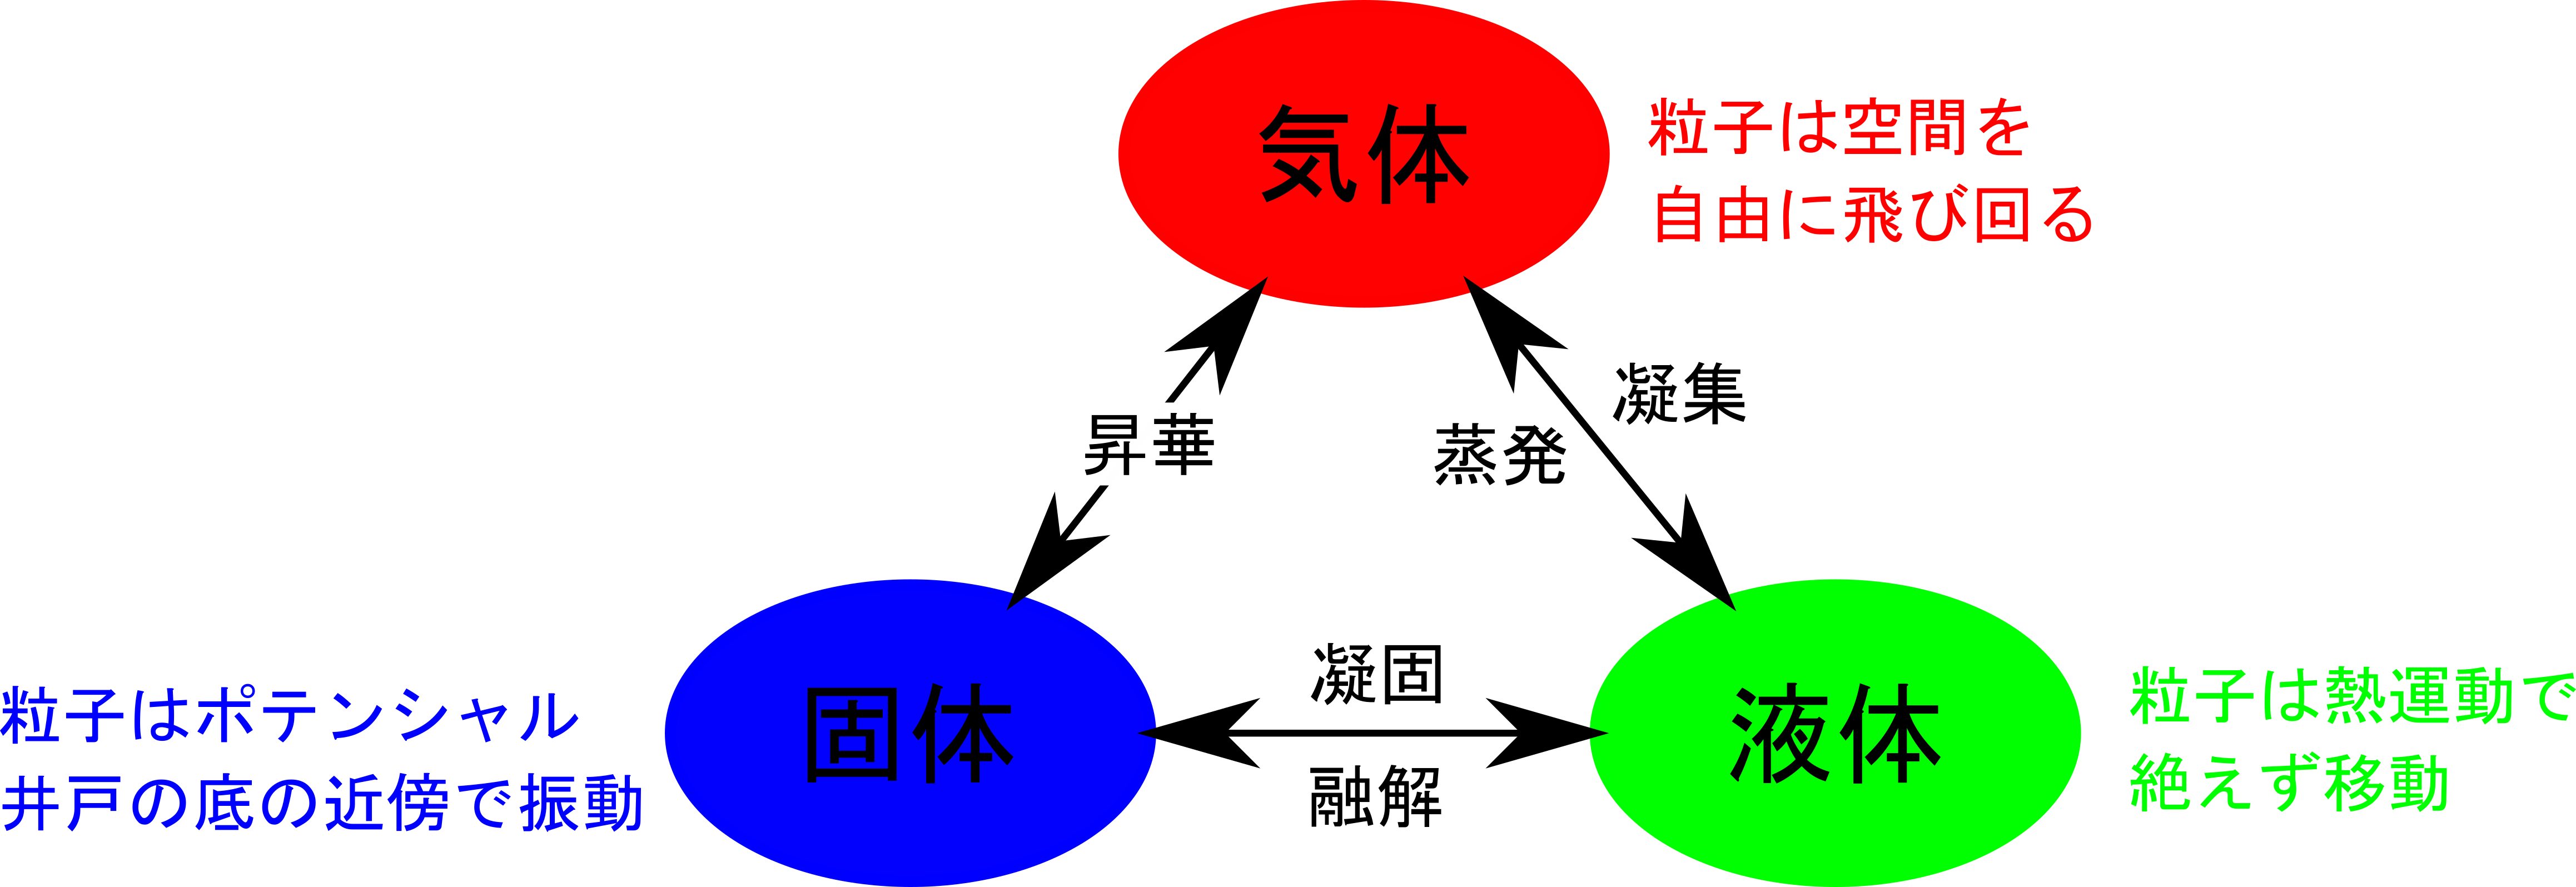
\includegraphics[width=\textwidth]{3Phase.png}
		\end{center}
\end{frame}

\begin{frame}
	\frametitle{マクロとミクロ}
		\begin{itemize}
			\item マクロな視点(手に取れるような大きさ)で考えると?
			\begin{itemize}
				\item 気体、液体 ⇔ 流れる、周りの形状に変形
				\item 固体 ⇔ 流れない、形を変えない
				\item 一言で言えば、「流れるかどうか?」\\
				(流れるということは、後ほど。)
			\end{itemize}
			\item \textcolor{red}{ミクロに中身を考えると何が違うのでしょうか?}
		\end{itemize}
		\begin{center}
			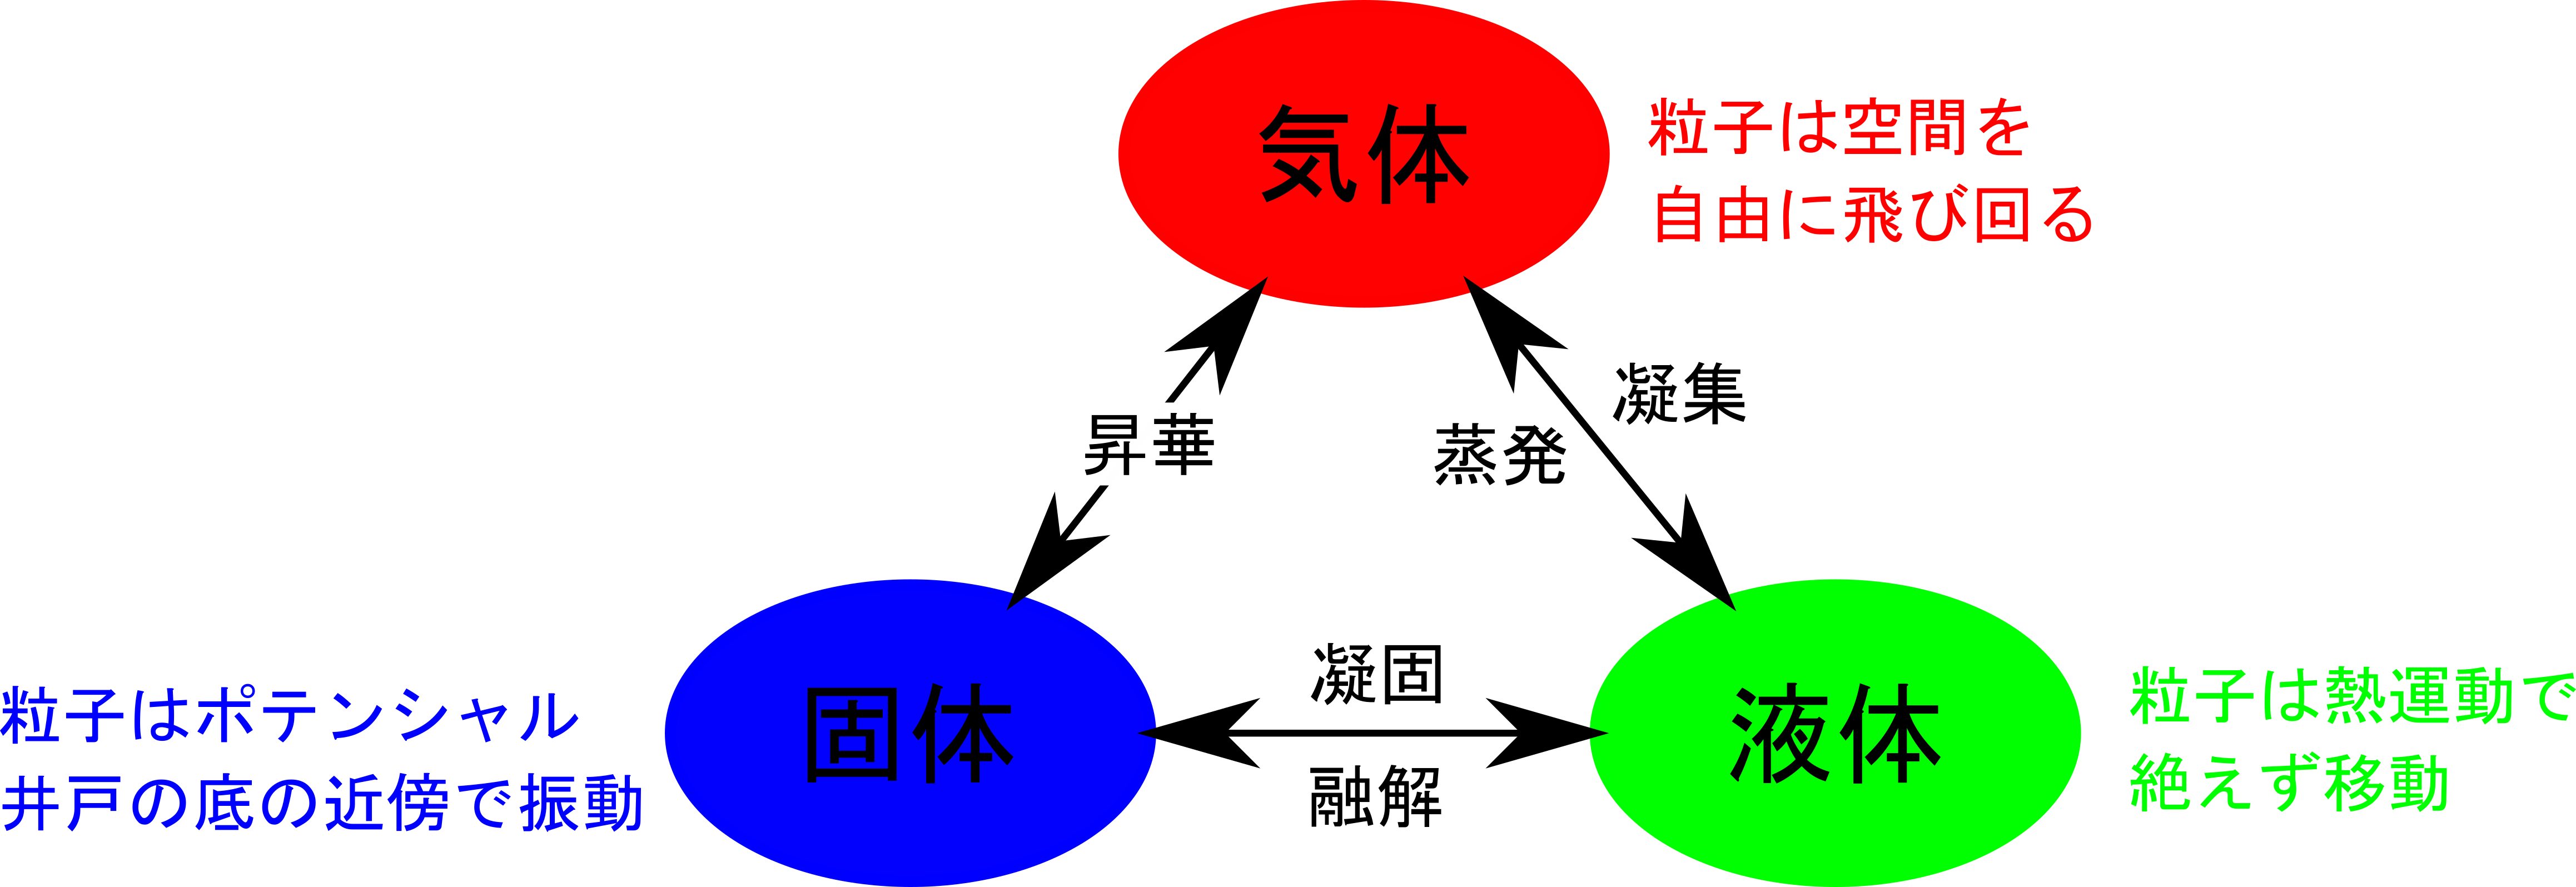
\includegraphics[width=\textwidth]{3Phase.png}
		\end{center}
\end{frame}


\subsection{固体のモデルとしての結晶}
\begin{frame}
	\frametitle{よくある個体の模式図}
		\begin{itemize}
			\item 固体の分類\\
			金属、塩、鉱物(石)、セラミックス(陶器)、ガラス、\\木材、等々
			\item 何らかの粒子(原子や分子)が規則的に並んだ「結晶としてモデル化」される場合が多い。
		\end{itemize}
		\begin{center}
			
\includegraphics[width=\textwidth]{crystals.png}
			固体のモデルとしての結晶(金属は省略)
		\end{center}
\end{frame}

\begin{frame}
	\frametitle{固体での粒子の関係}
	\begin{columns}[T, onlytextwidth]
		\column{.48\linewidth}
			\begin{exampleblock}{固体の粒子}
				\begin{itemize}
					\item 固体には、マクロな\\「流れないという性質」
					\item ミクロに見れば、粒子間に強い相互作用が必要
					% \item モデル化して考えれば、砂山は簡単に崩れますよね。
				\end{itemize}
			\end{exampleblock}
			\begin{center}
				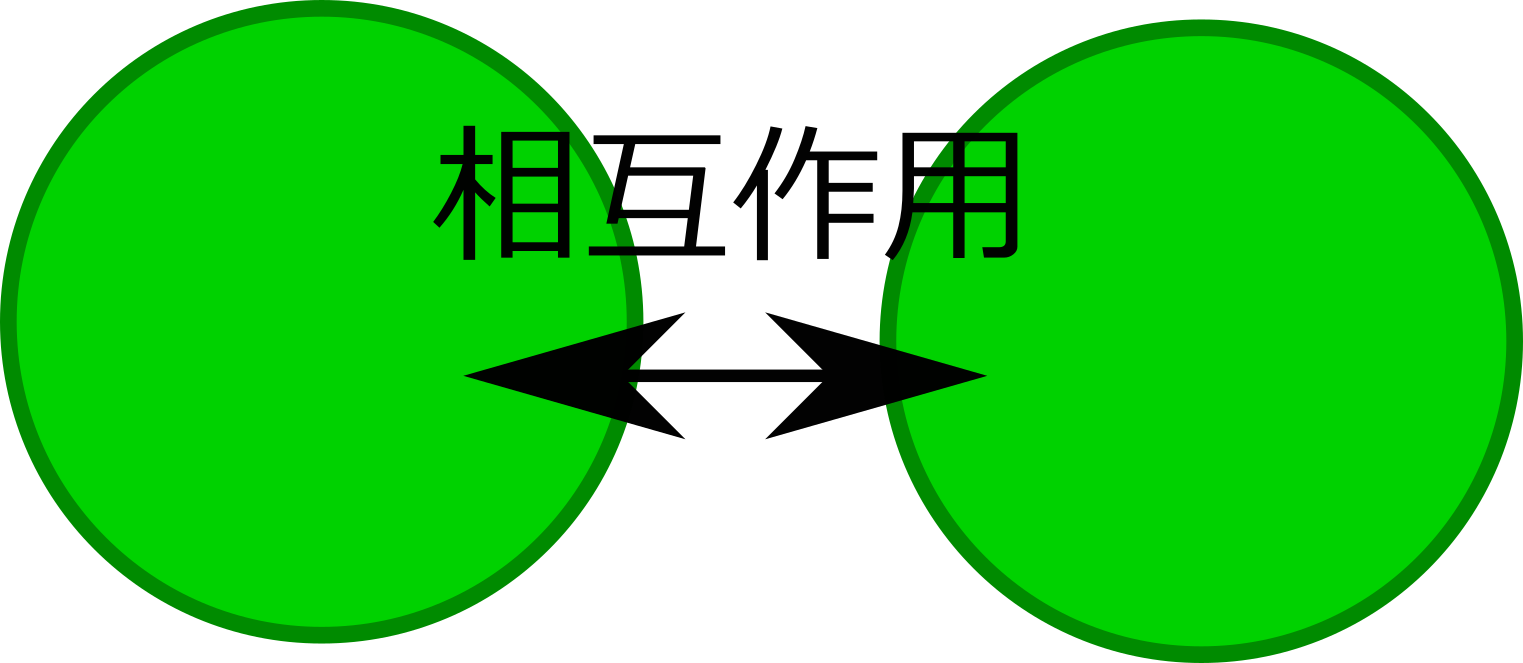
\includegraphics[width=\textwidth]{ryusi_1.png}
			\end{center}
		\column{.48\linewidth}
			\begin{block}{Lennard-Jones ポテンシャル}
				\begin{itemize}
					\item 速く消失する\textcolor{red}{斥力}
					\item 遠くまで働く\textcolor{blue}{引力}
					\item \textcolor{green}{それらの和}で相互作用
				\end{itemize}
				\vspace{-4mm}
				\scriptsize
				\begin{align*}
					U(r) = 4 \epsilon \left[ \textcolor{red}{\left(\dfrac{\sigma}{r} \right)^{12}} - \textcolor{blue}{\left(\dfrac{\sigma}{r} \right)^{6}} \right]
				\end{align*}
			\end{block}
			\vspace{-3mm}
				\begin{center}
					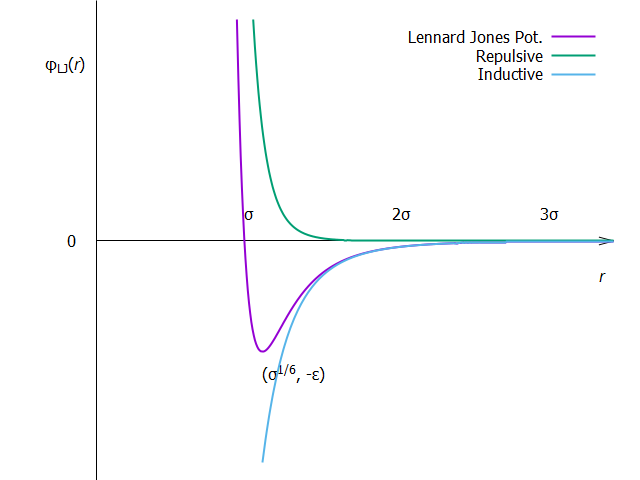
\includegraphics[width=.9\textwidth]{LJ_potential.png}
				\end{center}
	\end{columns}
\end{frame}

\begin{frame}
	\frametitle{LJ ポテンシャルと力}
	ポテンシャルを微分すると粒子間に働く力がわかります。
	\small
	\begin{align*}
		\begin{cases}
			U(r) = 4 \epsilon \left[ \left(\dfrac{\sigma}{r} \right)^{12} - \left(\dfrac{\sigma}{r} \right)^{6} \right] \\
			F(r) = -\dfrac{\rmd}{\rmd r}U(r) = 4 \epsilon \left[ 12 \left(\dfrac{\sigma^{12}}{r^{13}} \right) - 6 \left(\dfrac{\sigma^6}{r^7} \right) \right]
		\end{cases}
	\end{align*}
		\begin{center}
			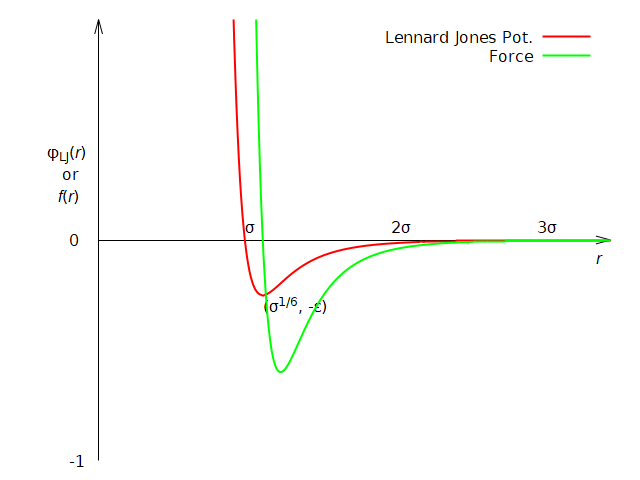
\includegraphics[width=.6\textwidth]{LJ_pot_Force.png}
		\end{center}
\end{frame}

\begin{frame}
	\frametitle{多数の粒子では}
		\begin{columns}[T, onlytextwidth]
			\column{.48\linewidth}
				\begin{block}{二体間の距離}
					\begin{itemize}
						\item 粒子の近接では斥力
						\item 離れすぎると引力
						\item その結果として、二粒子間の距離がほぼ定まる
					\end{itemize}
				\end{block}
				\begin{center}
					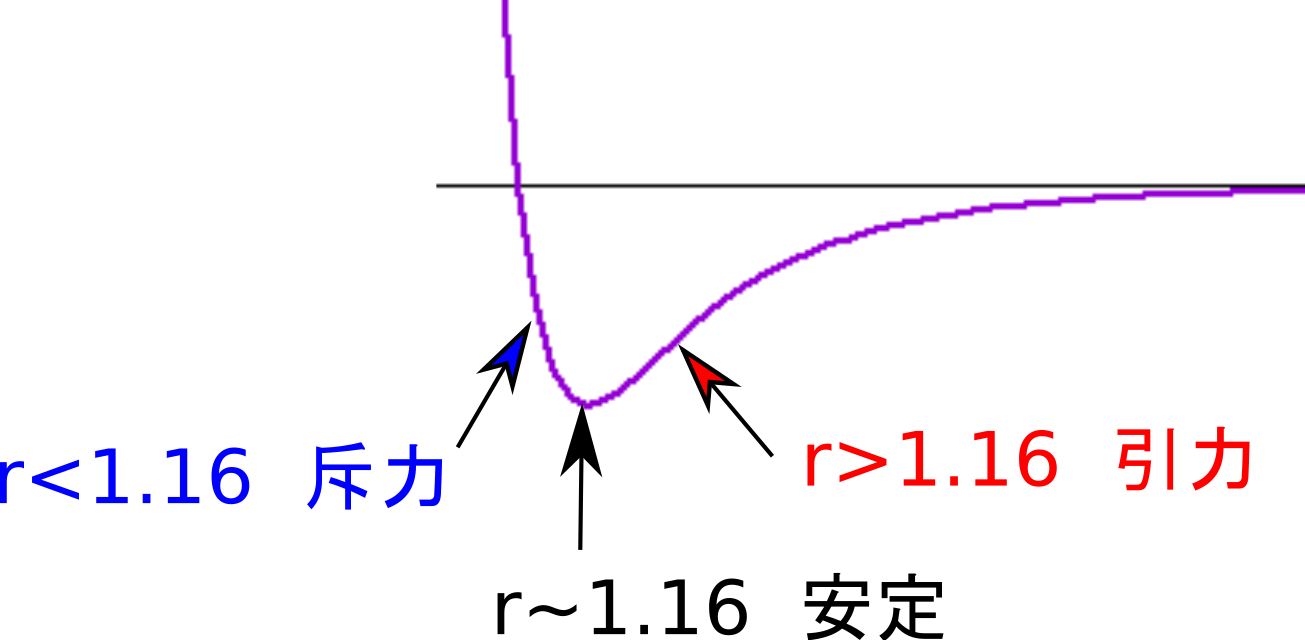
\includegraphics[width=\textwidth]{LJ_pos.png}
				\end{center}
			\column{.48\linewidth}
				\begin{exampleblock}{多体では}
					\begin{itemize}
						\item 二体間の相互作用により、
						\item 多体の粒子が安定距離の近傍で摂動
					\end{itemize}
				\end{exampleblock}
				\begin{center}
					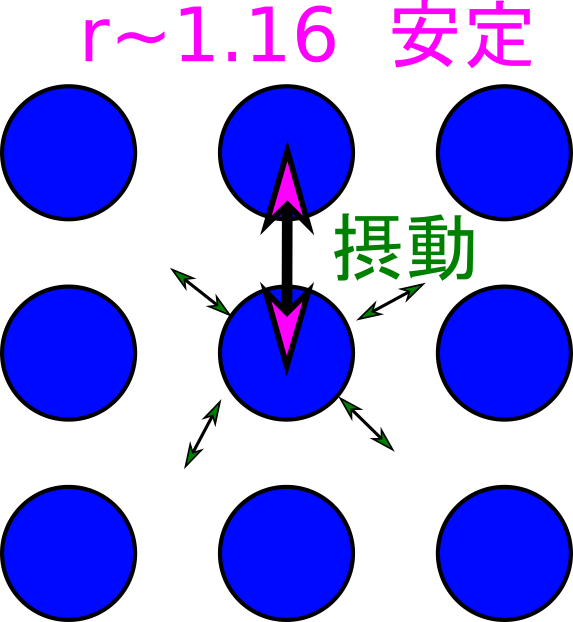
\includegraphics[width=.6\textwidth]{LJ_ryusi.png}
				\end{center}
		\end{columns}
\end{frame}

\begin{frame}
	\frametitle{固体のイメージ}
		\begin{columns}[T, onlytextwidth]
			\column{.48\linewidth}
				\begin{exampleblock}{分子動力学シミュレーション}
					\begin{itemize}
						\item 粒子の描像で物理現象をシミュレート
						\item それぞれの粒子の運動は、ニュートン力学に従う。
						\item 系の温度が粒子の揺動となる。
						\item 粒子の間に適切なポテンシャルを設定。
					\end{itemize}
				\end{exampleblock}
			\column{.48\linewidth}
				\begin{block}{固体のシミュレーション}
					\begin{itemize}
						\item T=0.1 (十分に低温)
						\item 面心立方になるように、\\初期の粒子を配置。
						\item 粒子の動きが少ない。
					\end{itemize}
				\end{block}
				\begin{center}
					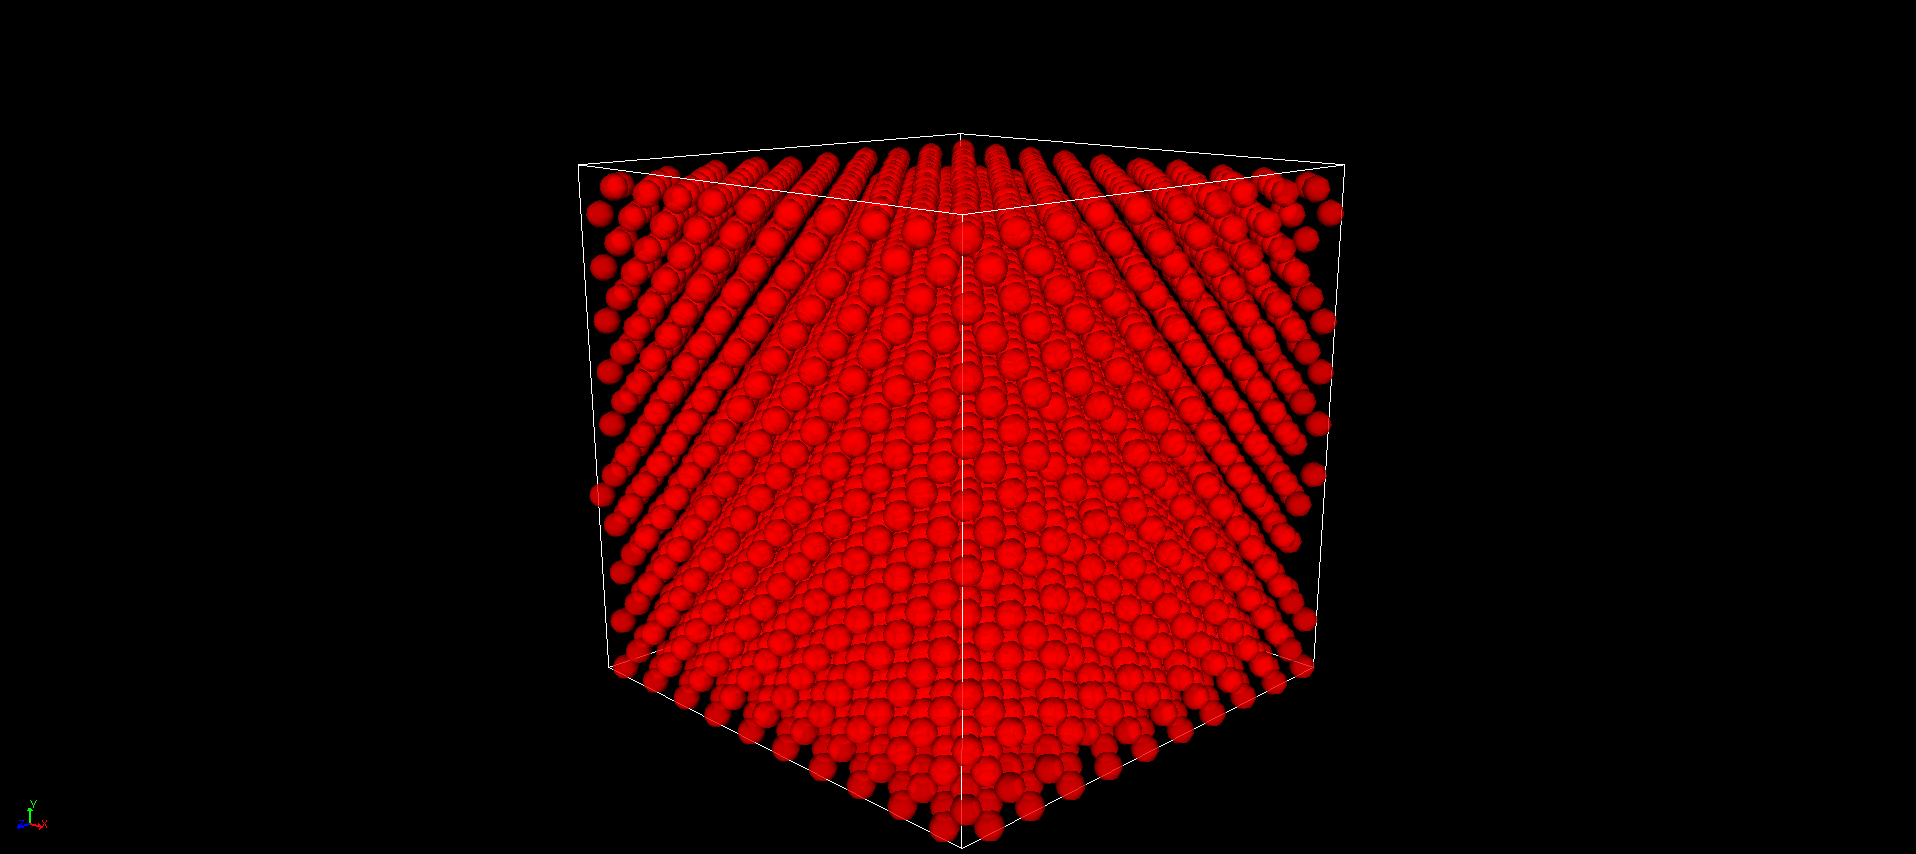
\includegraphics[width=\textwidth]{N1_FCC.png}
				\textcolor{red}{これはスナップショット、\\動画でも殆ど動いていない。}
				\end{center}
		\end{columns}
\end{frame}

\subsection{固体と液体}
\begin{frame}
	\frametitle{固体と液体の間にある相転移}
	\begin{columns}[T, onlytextwidth]
		\column{.48\linewidth}
		\begin{block}{マクロに見れば}
			\begin{itemize}
				\item 融解、結晶時に、比熱や体積に「飛び」が発生。
				\item 内部のパッキングが緩む。
			\end{itemize}
		\end{block}
		\begin{center}
			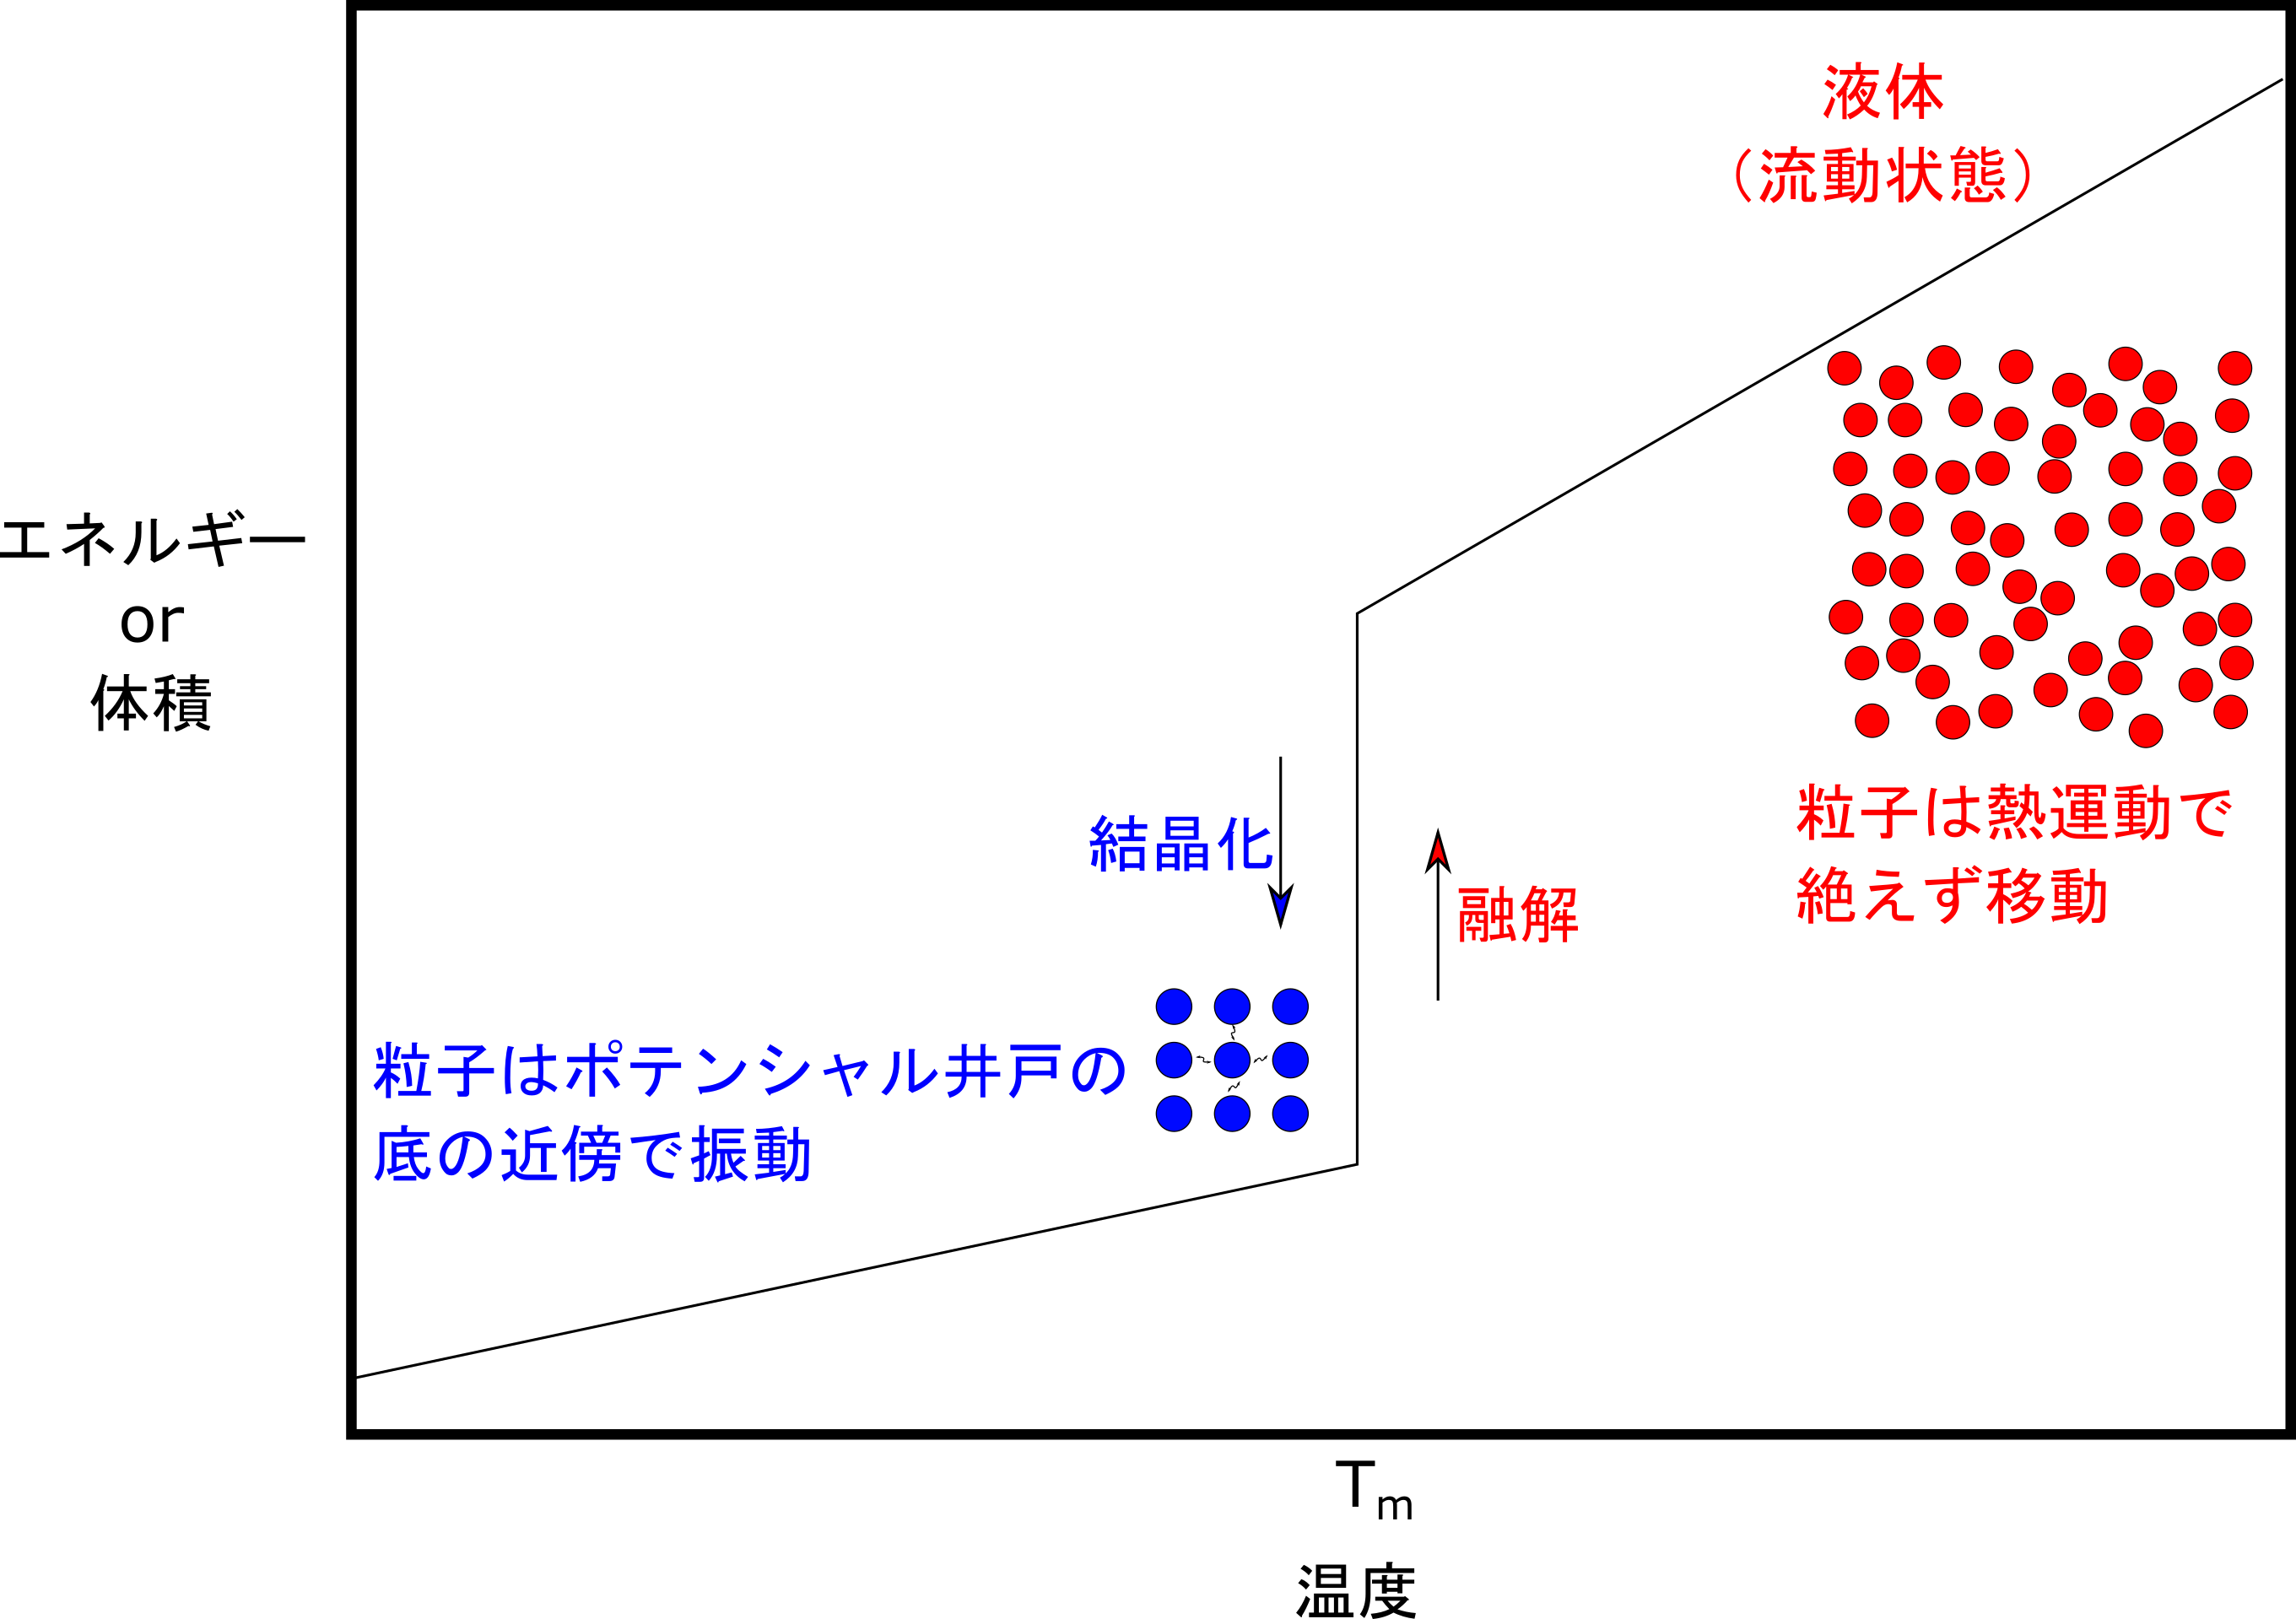
\includegraphics[width=\textwidth]{crystal_melt.png}
		\end{center}
		\column{.48\linewidth}
			\begin{exampleblock}{ミクロに見ると}
				\begin{itemize}
					\item 粒子の摂動が増加
					\item 粒子間の距離が伸びる
					\item MD シミュレーションでの液体のイメージ(T=1.0)
				\end{itemize}
				\begin{center}
					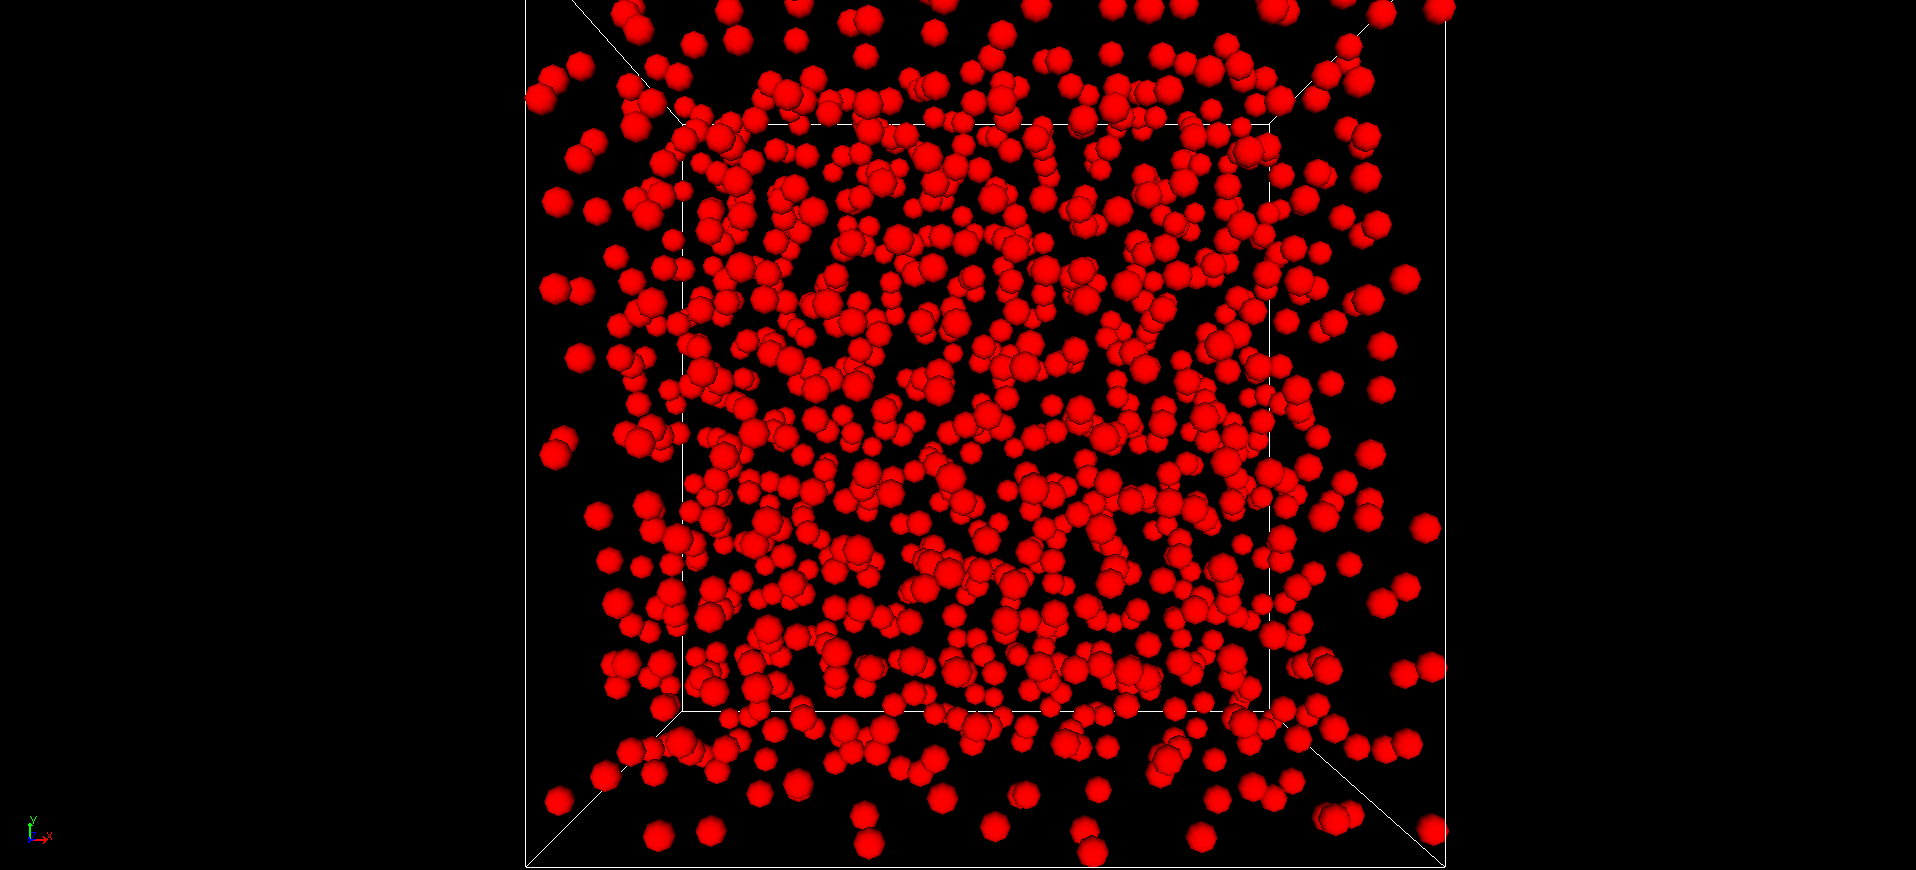
\includegraphics[width=\textwidth]{N1_Melt.png}
					\href{https://drive.google.com/file/d/1ceUaJomvBvljykBGIyLaRJXQbGJzlGUm/view?usp=sharing}{\textcolor{red}{動画へのリンク}}
				\end{center}
			\end{exampleblock}
	\end{columns}
\end{frame}

\begin{frame}
	\frametitle{粒子間の状態を観る方法}
	\begin{columns}[T, onlytextwidth]
		\column{.48\linewidth}
			\begin{exampleblock}{動径分布関数:}
				\begin{itemize}
					\item ある粒子からみて、\\距離の関数として\\他粒子を数えあげる。
					\item すべての粒子で同じことをやる。
				\end{itemize}
			\end{exampleblock}
			\begin{center}
				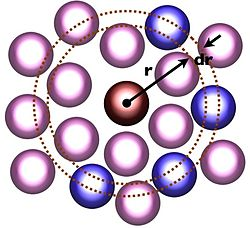
\includegraphics[width=.6\textwidth]{gr.jpg}
			\end{center}
		\column{.48\linewidth}
			\begin{block}{シミュレーションの結果}
				\begin{itemize}
					\item 固体の動径分布関数
					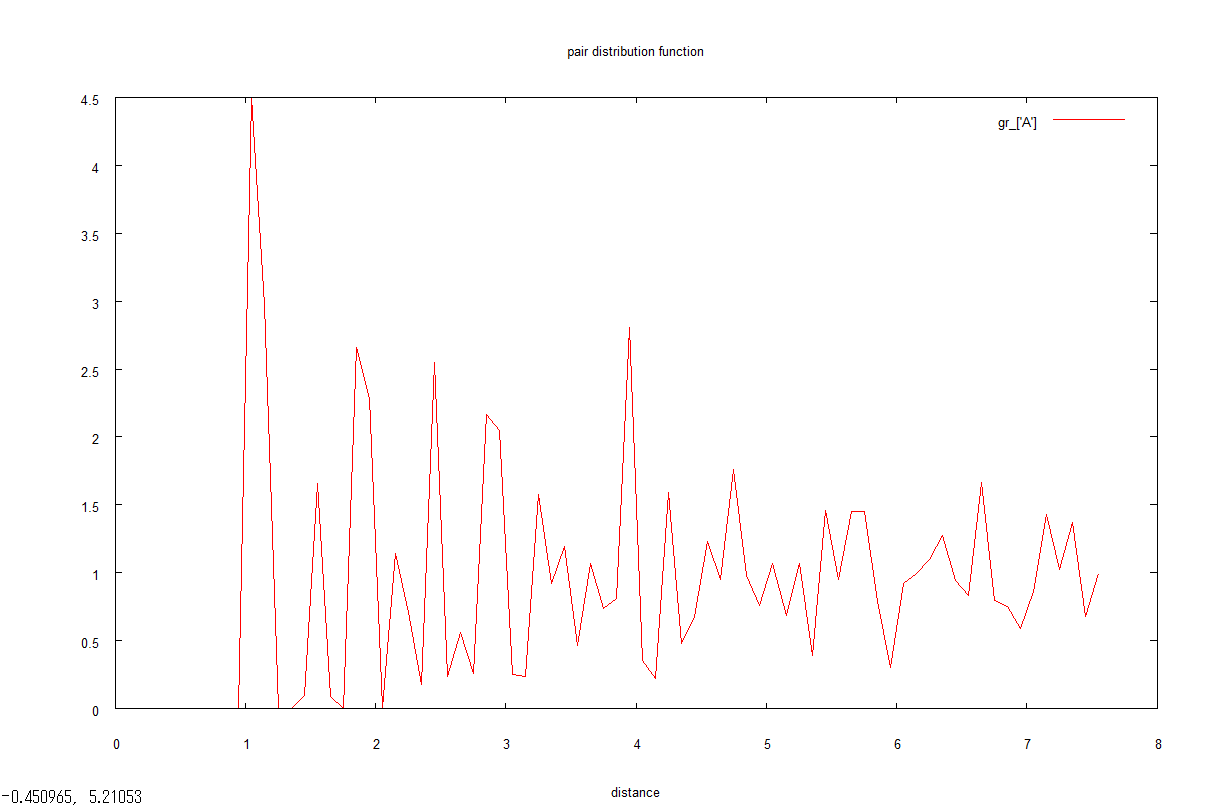
\includegraphics[width=.7\textwidth]{Gr_N1_Cry_T_0_1.png}
					\item 液体の動径分布関数
					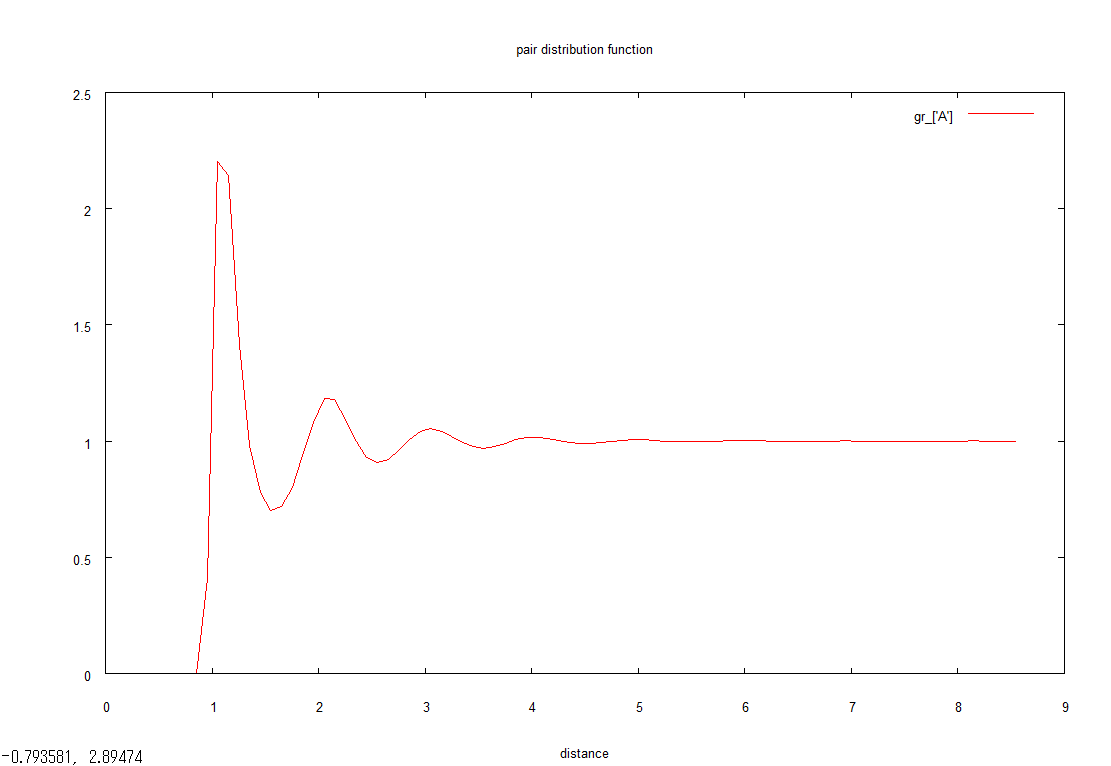
\includegraphics[width=.7\textwidth]{Gr_N1_Cry_T_1.png}
				\end{itemize}
			\end{block}
	\end{columns}
\end{frame}

\begin{frame}
	\frametitle{液体の空隙と粒子の移動}
		\begin{columns}[T, onlytextwidth]
			\column{.48\linewidth}
				\begin{itemize}
					\item 液体の相互の位置は、規則的ではない。
					\item 粒子径(r/σ=1)より少し離れた所にピーク。
					\item それより少し遠くに、密度の低い領域が。
				\end{itemize}
					\begin{center}
						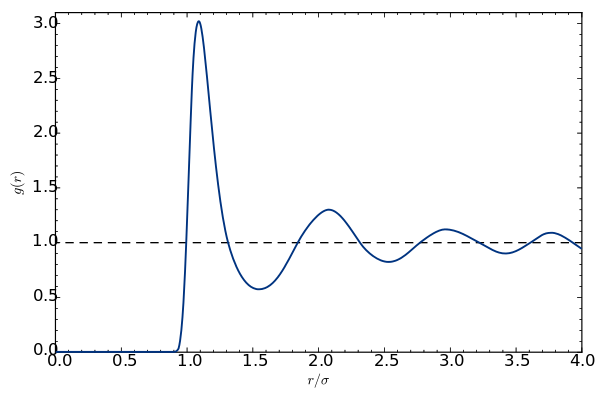
\includegraphics[width=\textwidth]{gr_2.png}
					\end{center}
			\column{.48\linewidth}
				\begin{exampleblock}{液体での粒子の移動}
					\begin{itemize}
						\item 乱雑に並んだ粒子がそれぞれ運動。
						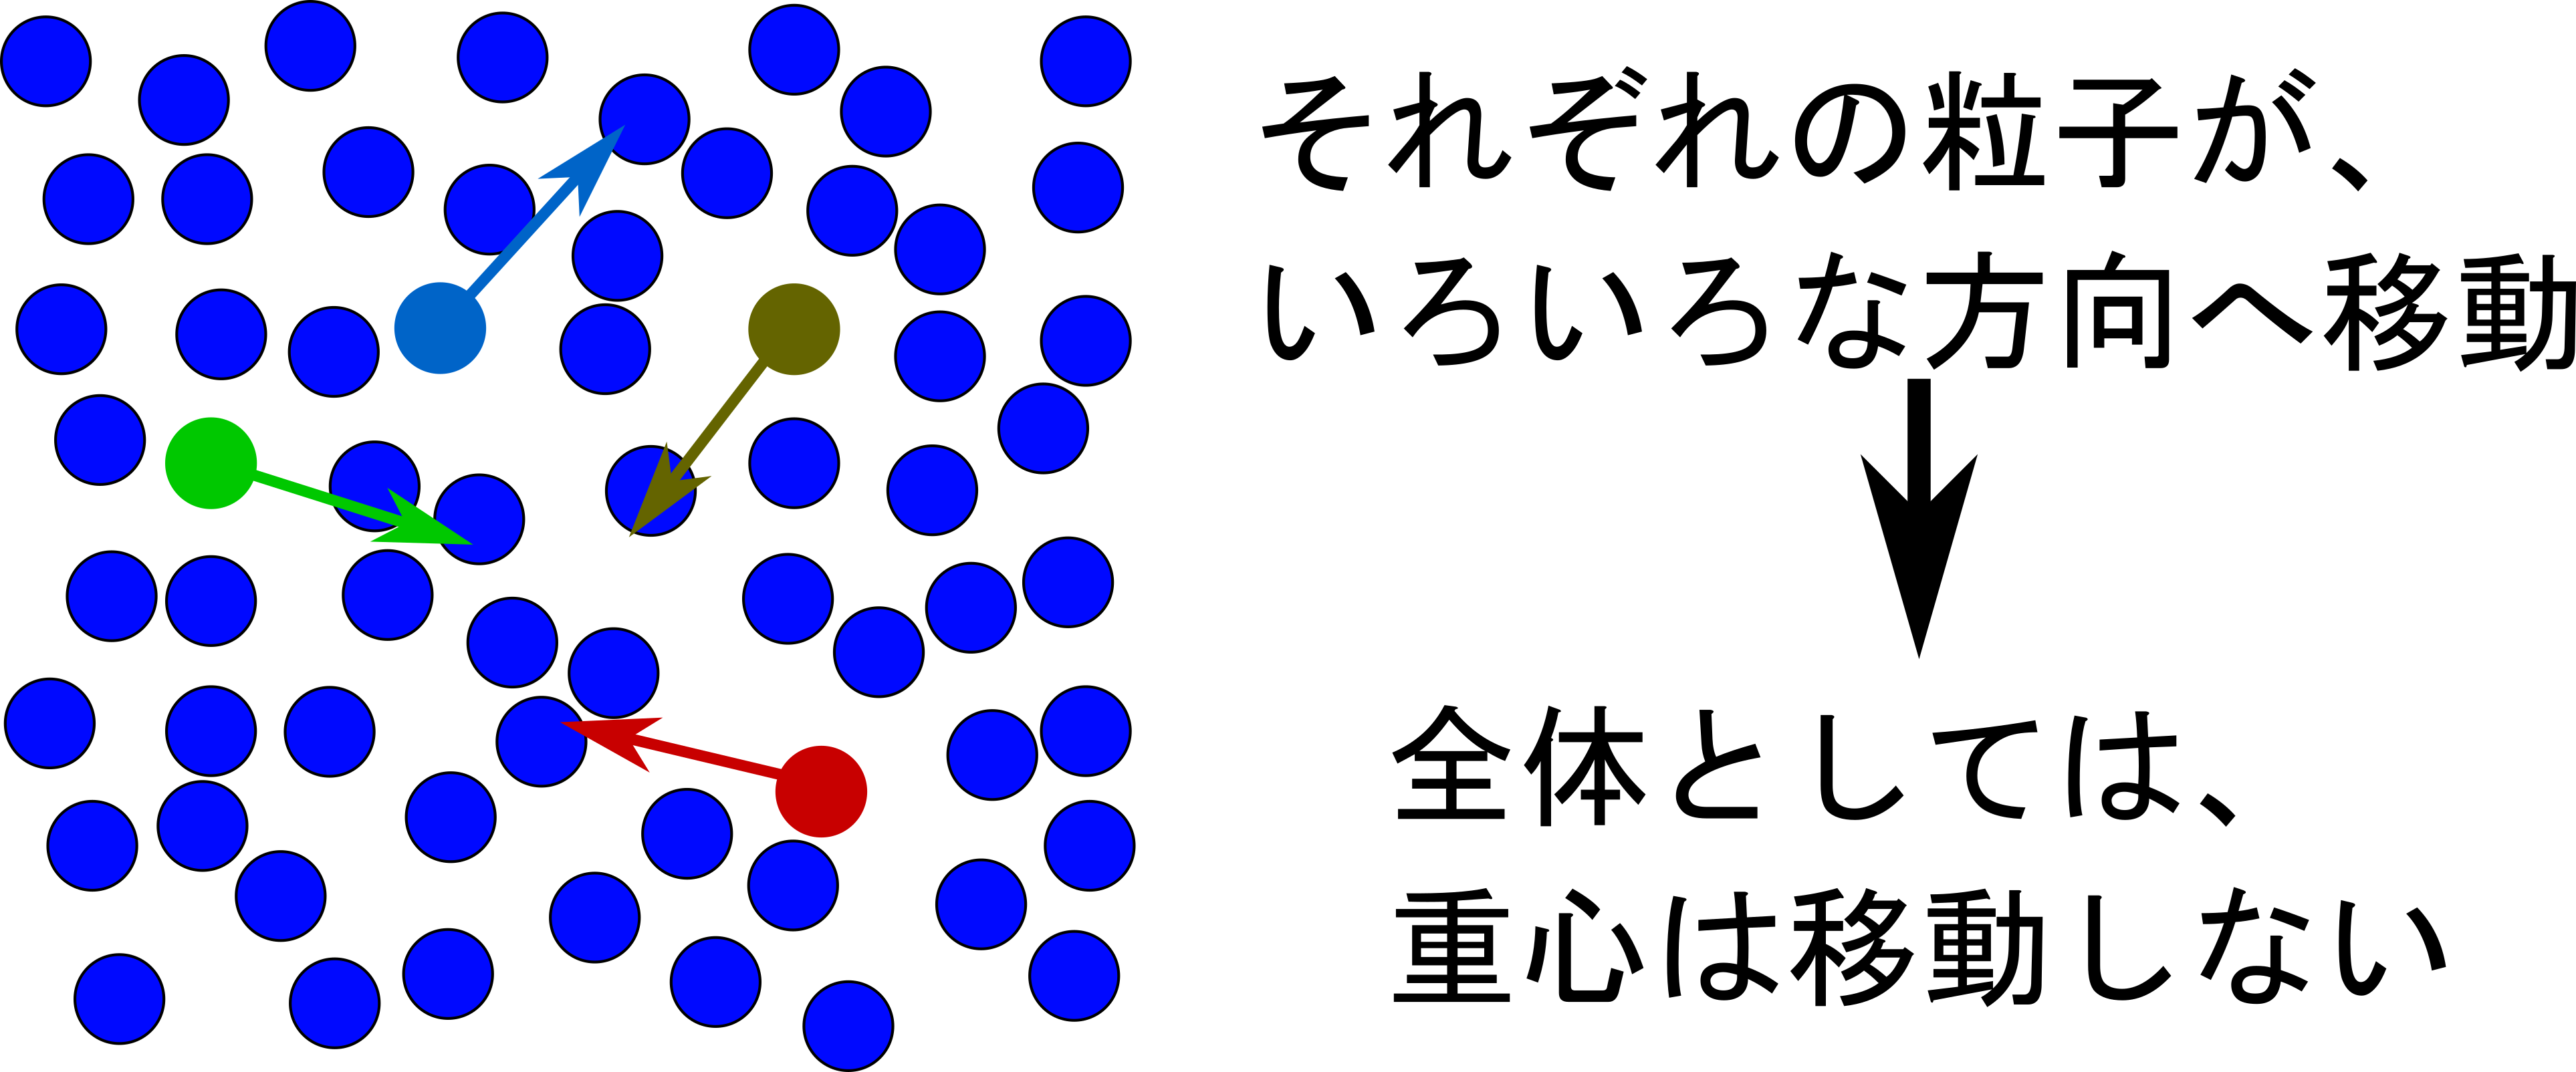
\includegraphics[width=.85\textwidth]{liquid_model.png}
						\item 一粒子に着目すると、少しずつ元の位置から移動
						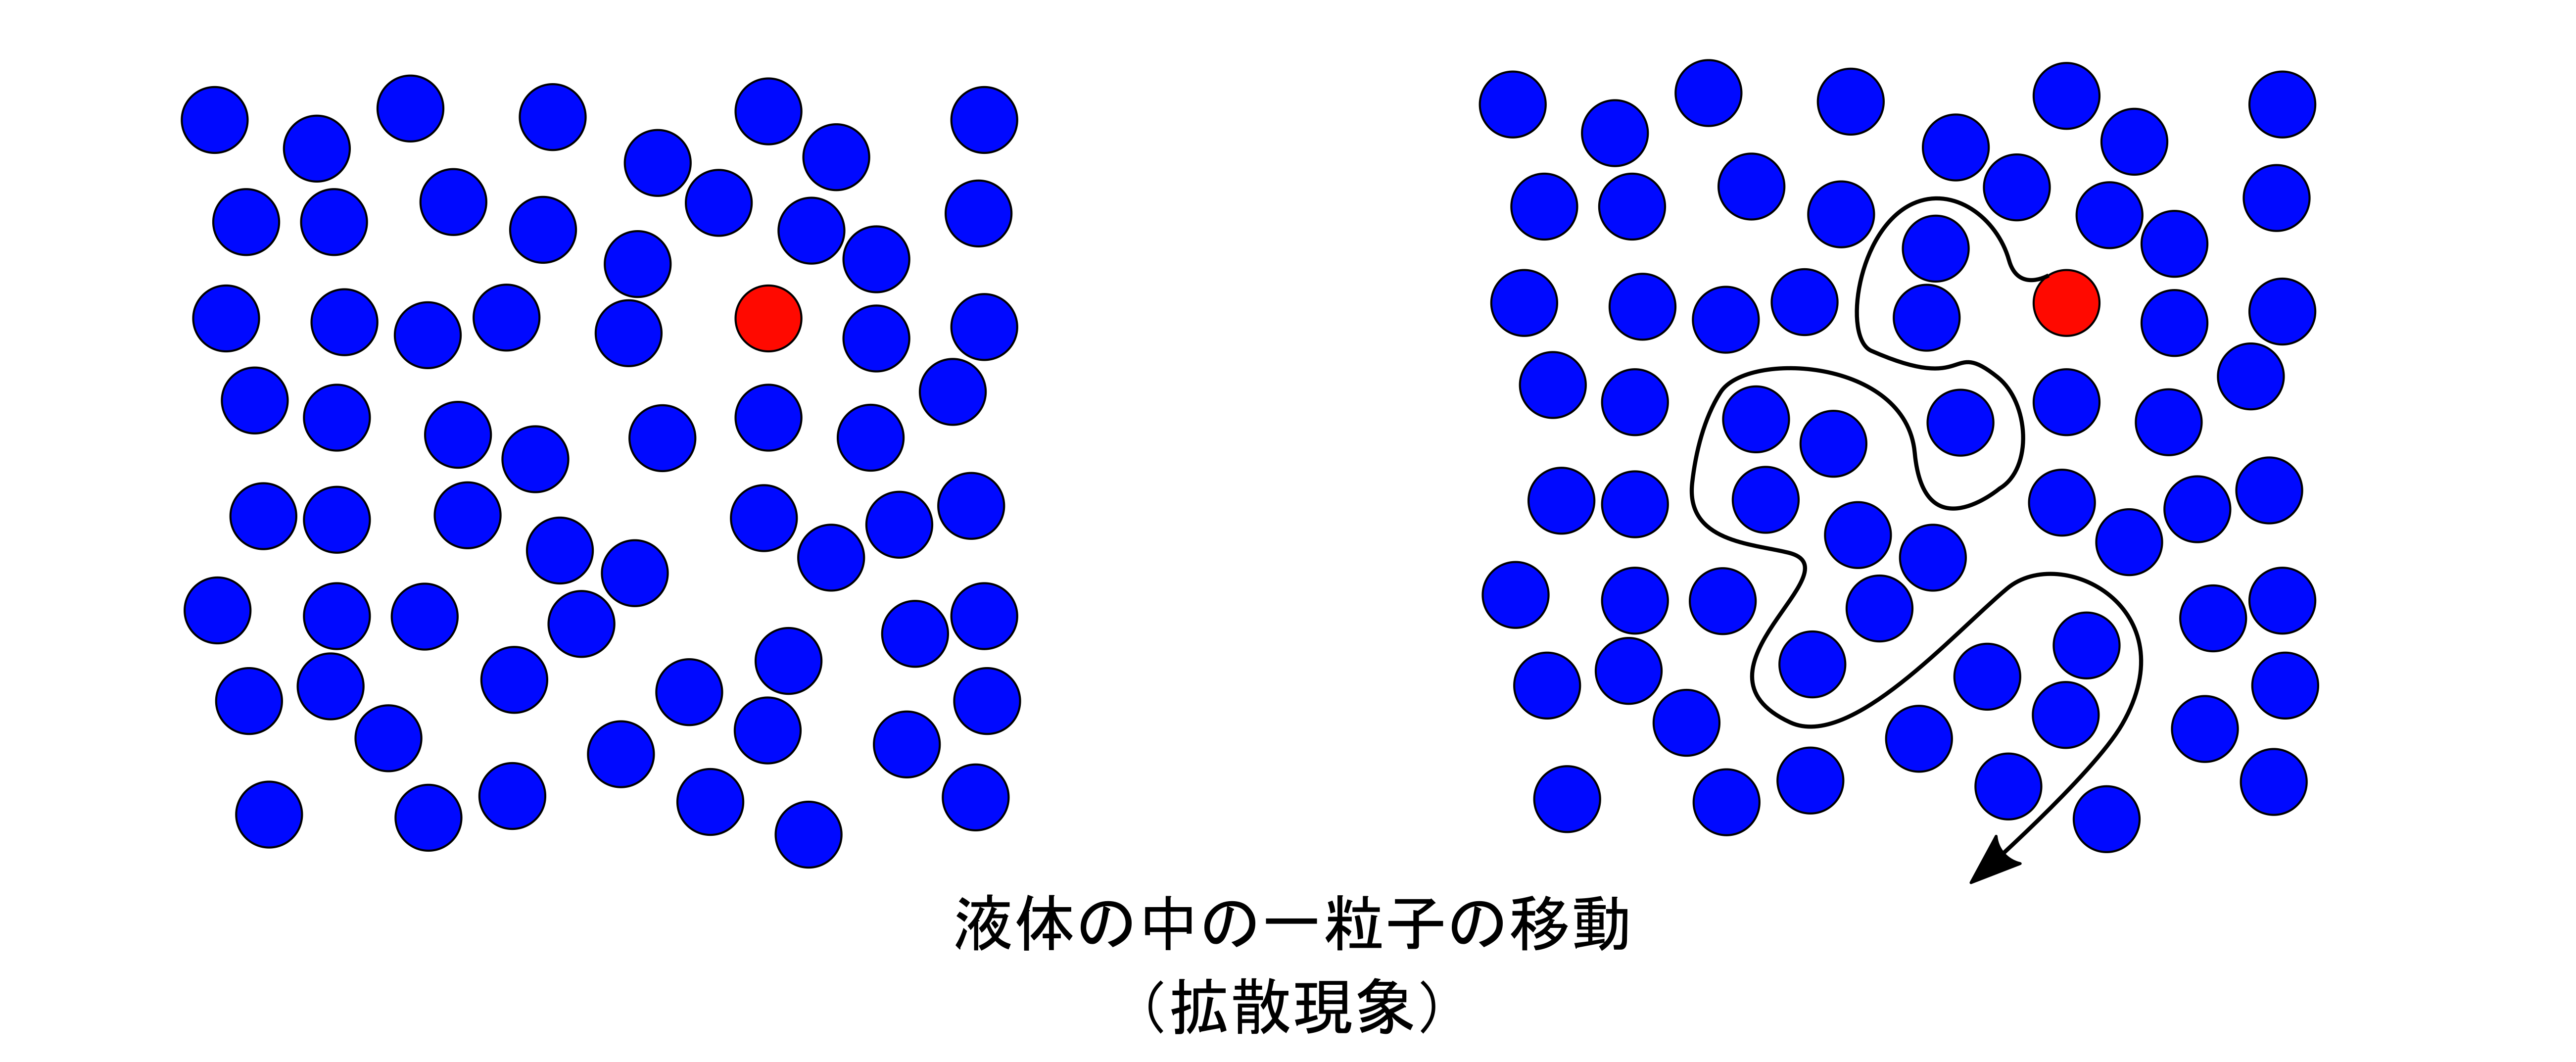
\includegraphics[width=.85\textwidth]{liquid_1.png}
					\end{itemize}
				\end{exampleblock}
		\end{columns}
\end{frame}

\begin{frame}
	\frametitle{マクロな描像とミクロにおきていること}	
		\begin{columns}[T, onlytextwidth]
			\column{.6\linewidth}
				\begin{exampleblock}{コップの中の水:外力を加えない時}
					\begin{itemize}
						\item マクロには、
						\begin{itemize}
							\item 変化しない:止まって見える
						\end{itemize}
						\item ミクロには、
						\begin{itemize}
							\item 熱エネルギーで粒子が\\ランダムに運動
							\item 粒子の近くに隙間ができると移動
							\item その移動により別の隙間が\\でき、他の粒子がそこに移動。
							\item 上記の相互の入れ替えは、\\常に発生。
						\end{itemize}
					\end{itemize}
				\end{exampleblock}
			\column{.36\linewidth}
					\begin{center}
						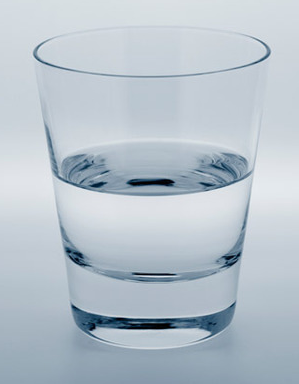
\includegraphics[width=.8\textwidth]{cup_water.png}

						\vspace{5mm}
						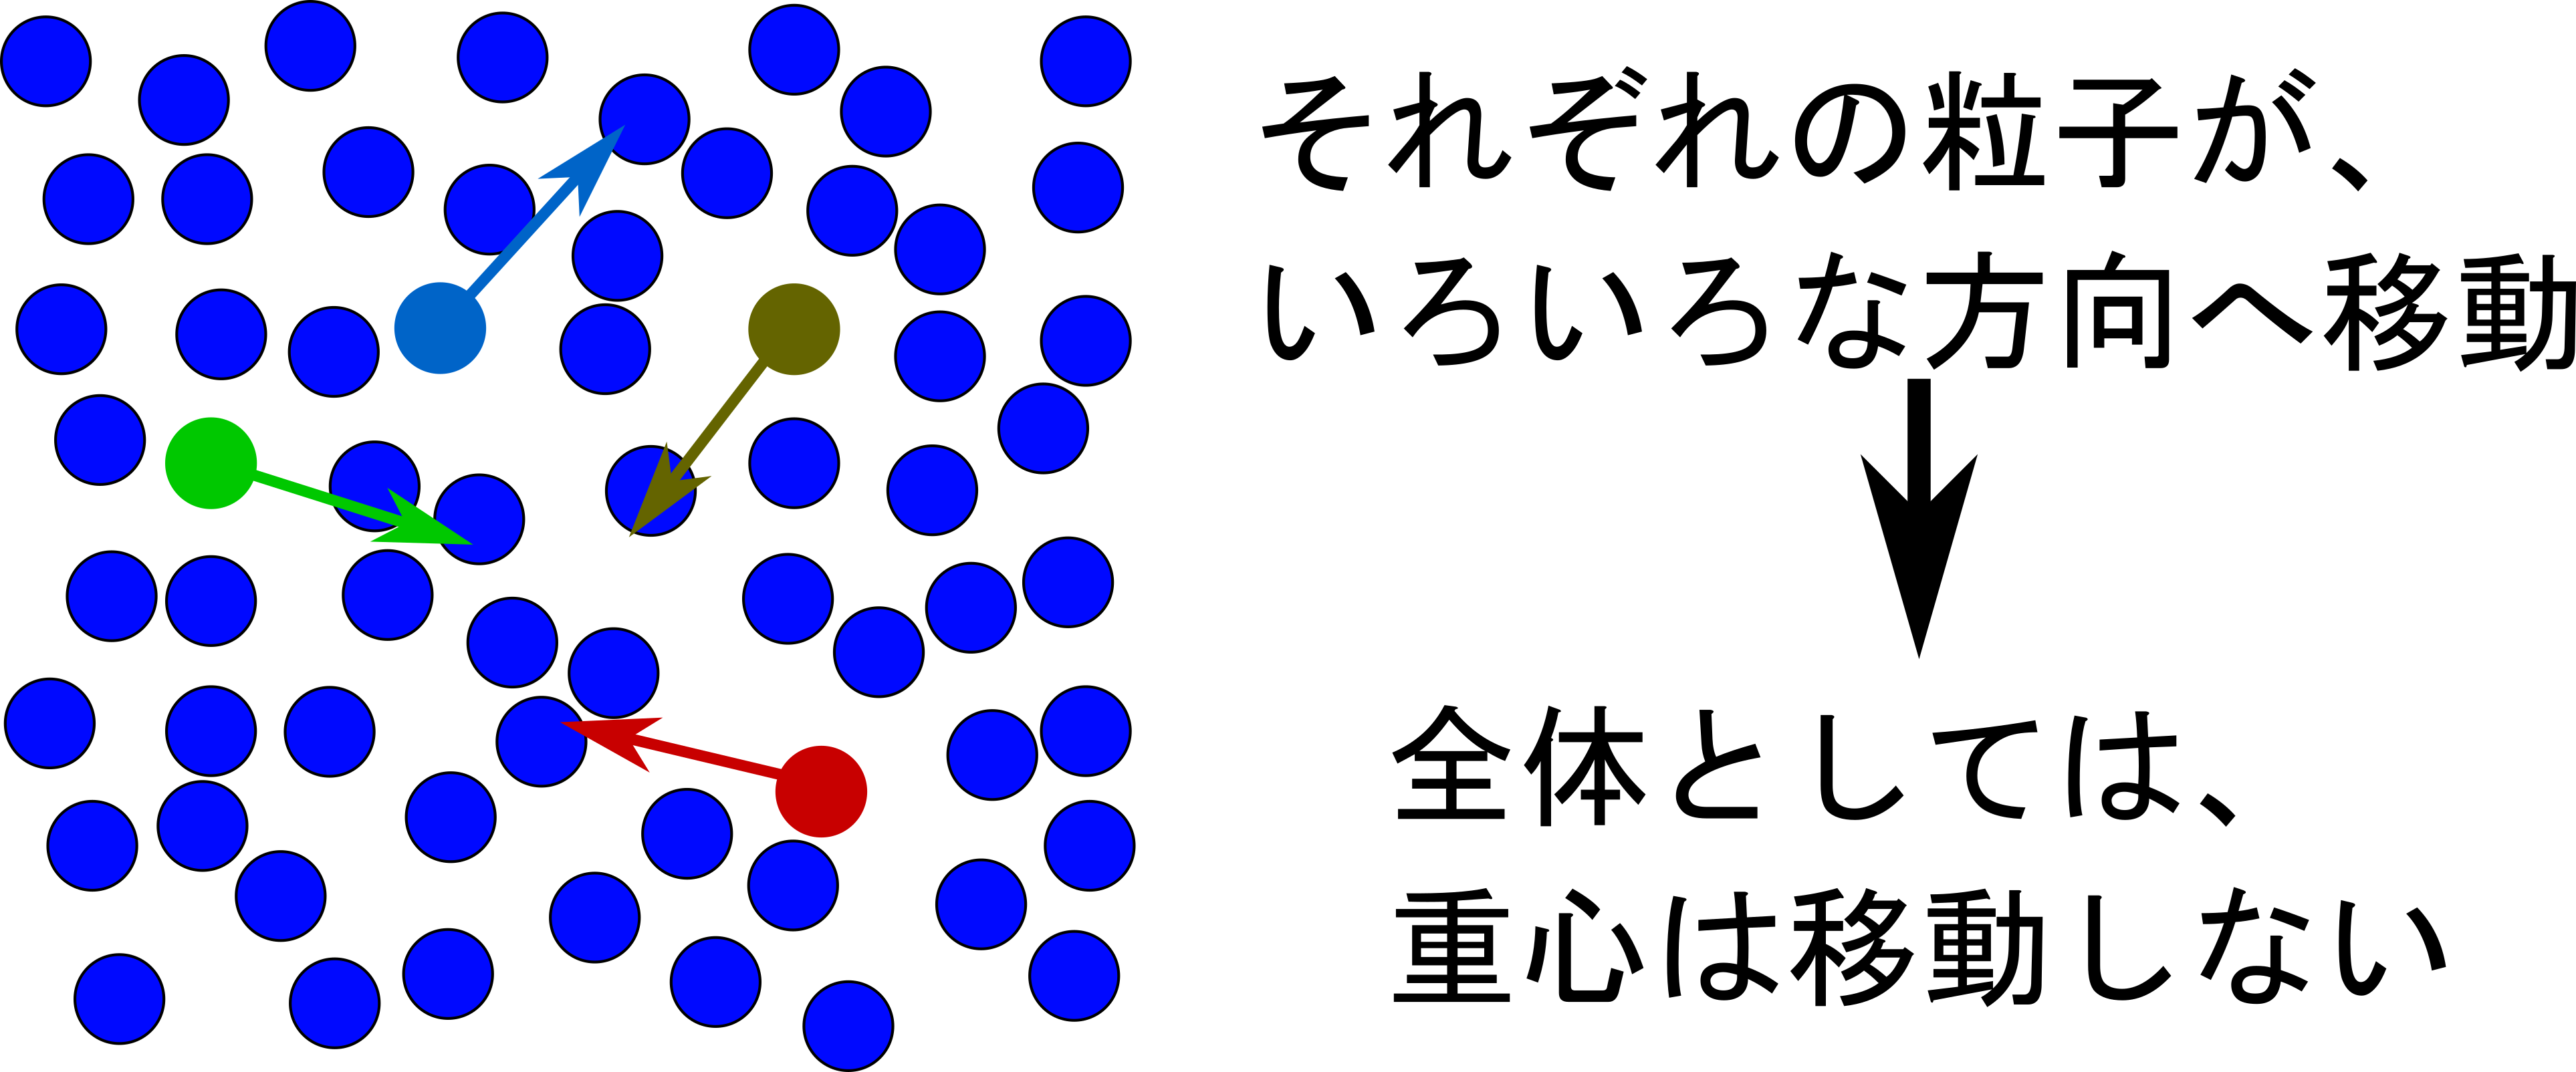
\includegraphics[width=\textwidth]{liquid_model.png}
					\end{center}
		\end{columns}
\end{frame}

\begin{frame}
	\frametitle{結局、物質の三態とは}
		\begin{columns}[T, onlytextwidth]
			\column{.46\linewidth}
				\begin{block}{温度ベースで考えると、}
					\begin{itemize}
						\item 高温では気体:\\
						粒子が自由に動ける
						\item 中温では液体:\\
						適度に移動できる
						\item 低温では固体:\\
						最も落ち着きのいい\\位置に留まる
					\end{itemize}
				\end{block}
					\begin{center}
						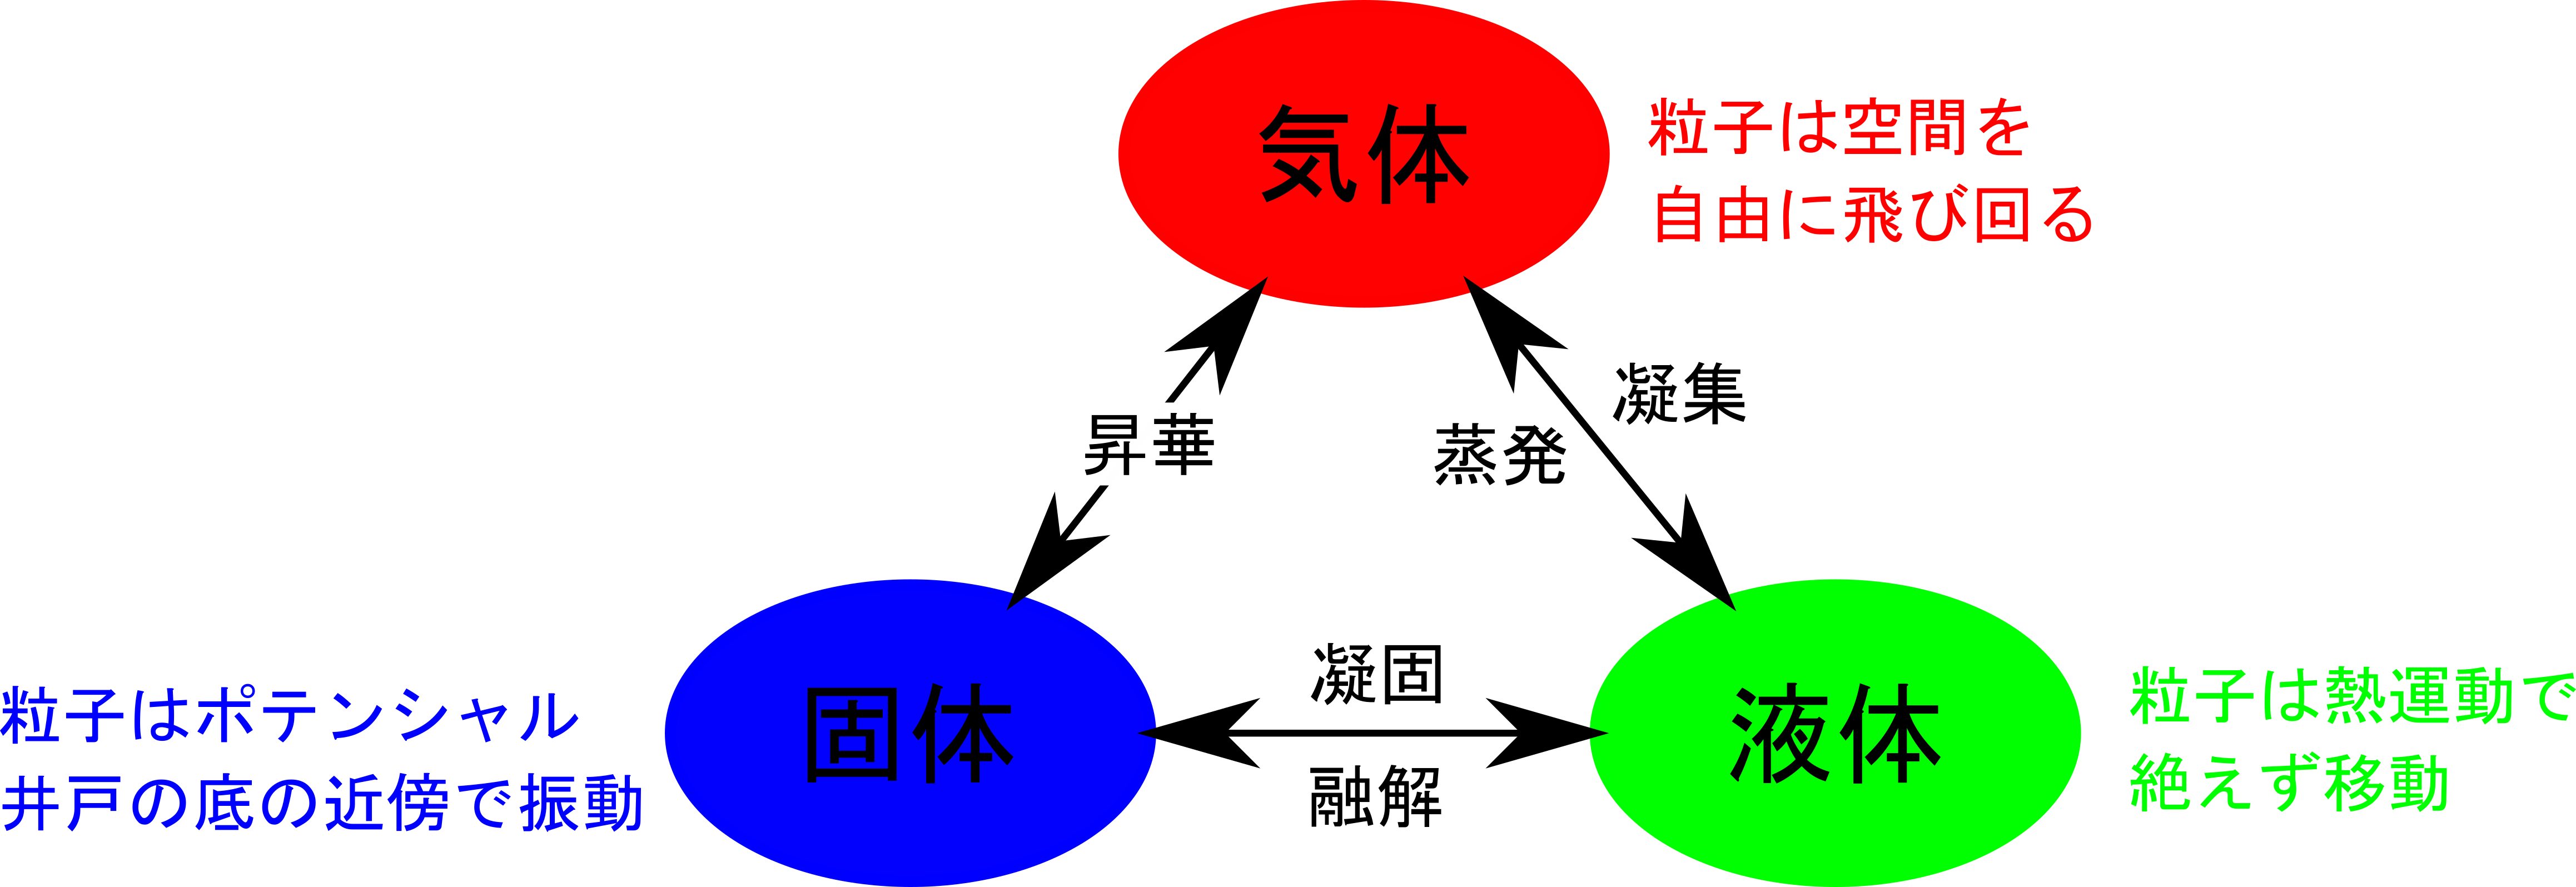
\includegraphics[width=\textwidth]{3Phase.png}
					\end{center}
			\column{.5\linewidth}
				\begin{exampleblock}{ミクロに二つのせめぎあい}
					\begin{itemize}
						\item 粒子は熱エネルギーで、\\揺らされる。
						\item 居心地のいい位置に。
					\end{itemize}
				\end{exampleblock}
				\vspace{-2mm}
				\begin{alertblock}{その結果として}
					\begin{itemize}
						\item 固体:相対的に揺動小
						\begin{itemize}
							\item ポテンシャル井戸の\\底近傍で振動
							\item 内部構造を形成。
						\end{itemize}
						\item 液体:熱揺動が大きい
						\begin{itemize}
							\item 多くの粒子が相互作用
							\item 構造が不定
						\end{itemize}
					\end{itemize}
				\end{alertblock}
		\end{columns}	
\end{frame}

\begin{frame}
	\frametitle{温度と相転移}
		これまでの考え方で、以下の液体と固体の相転移を、\\理解できます。
		\begin{center}
			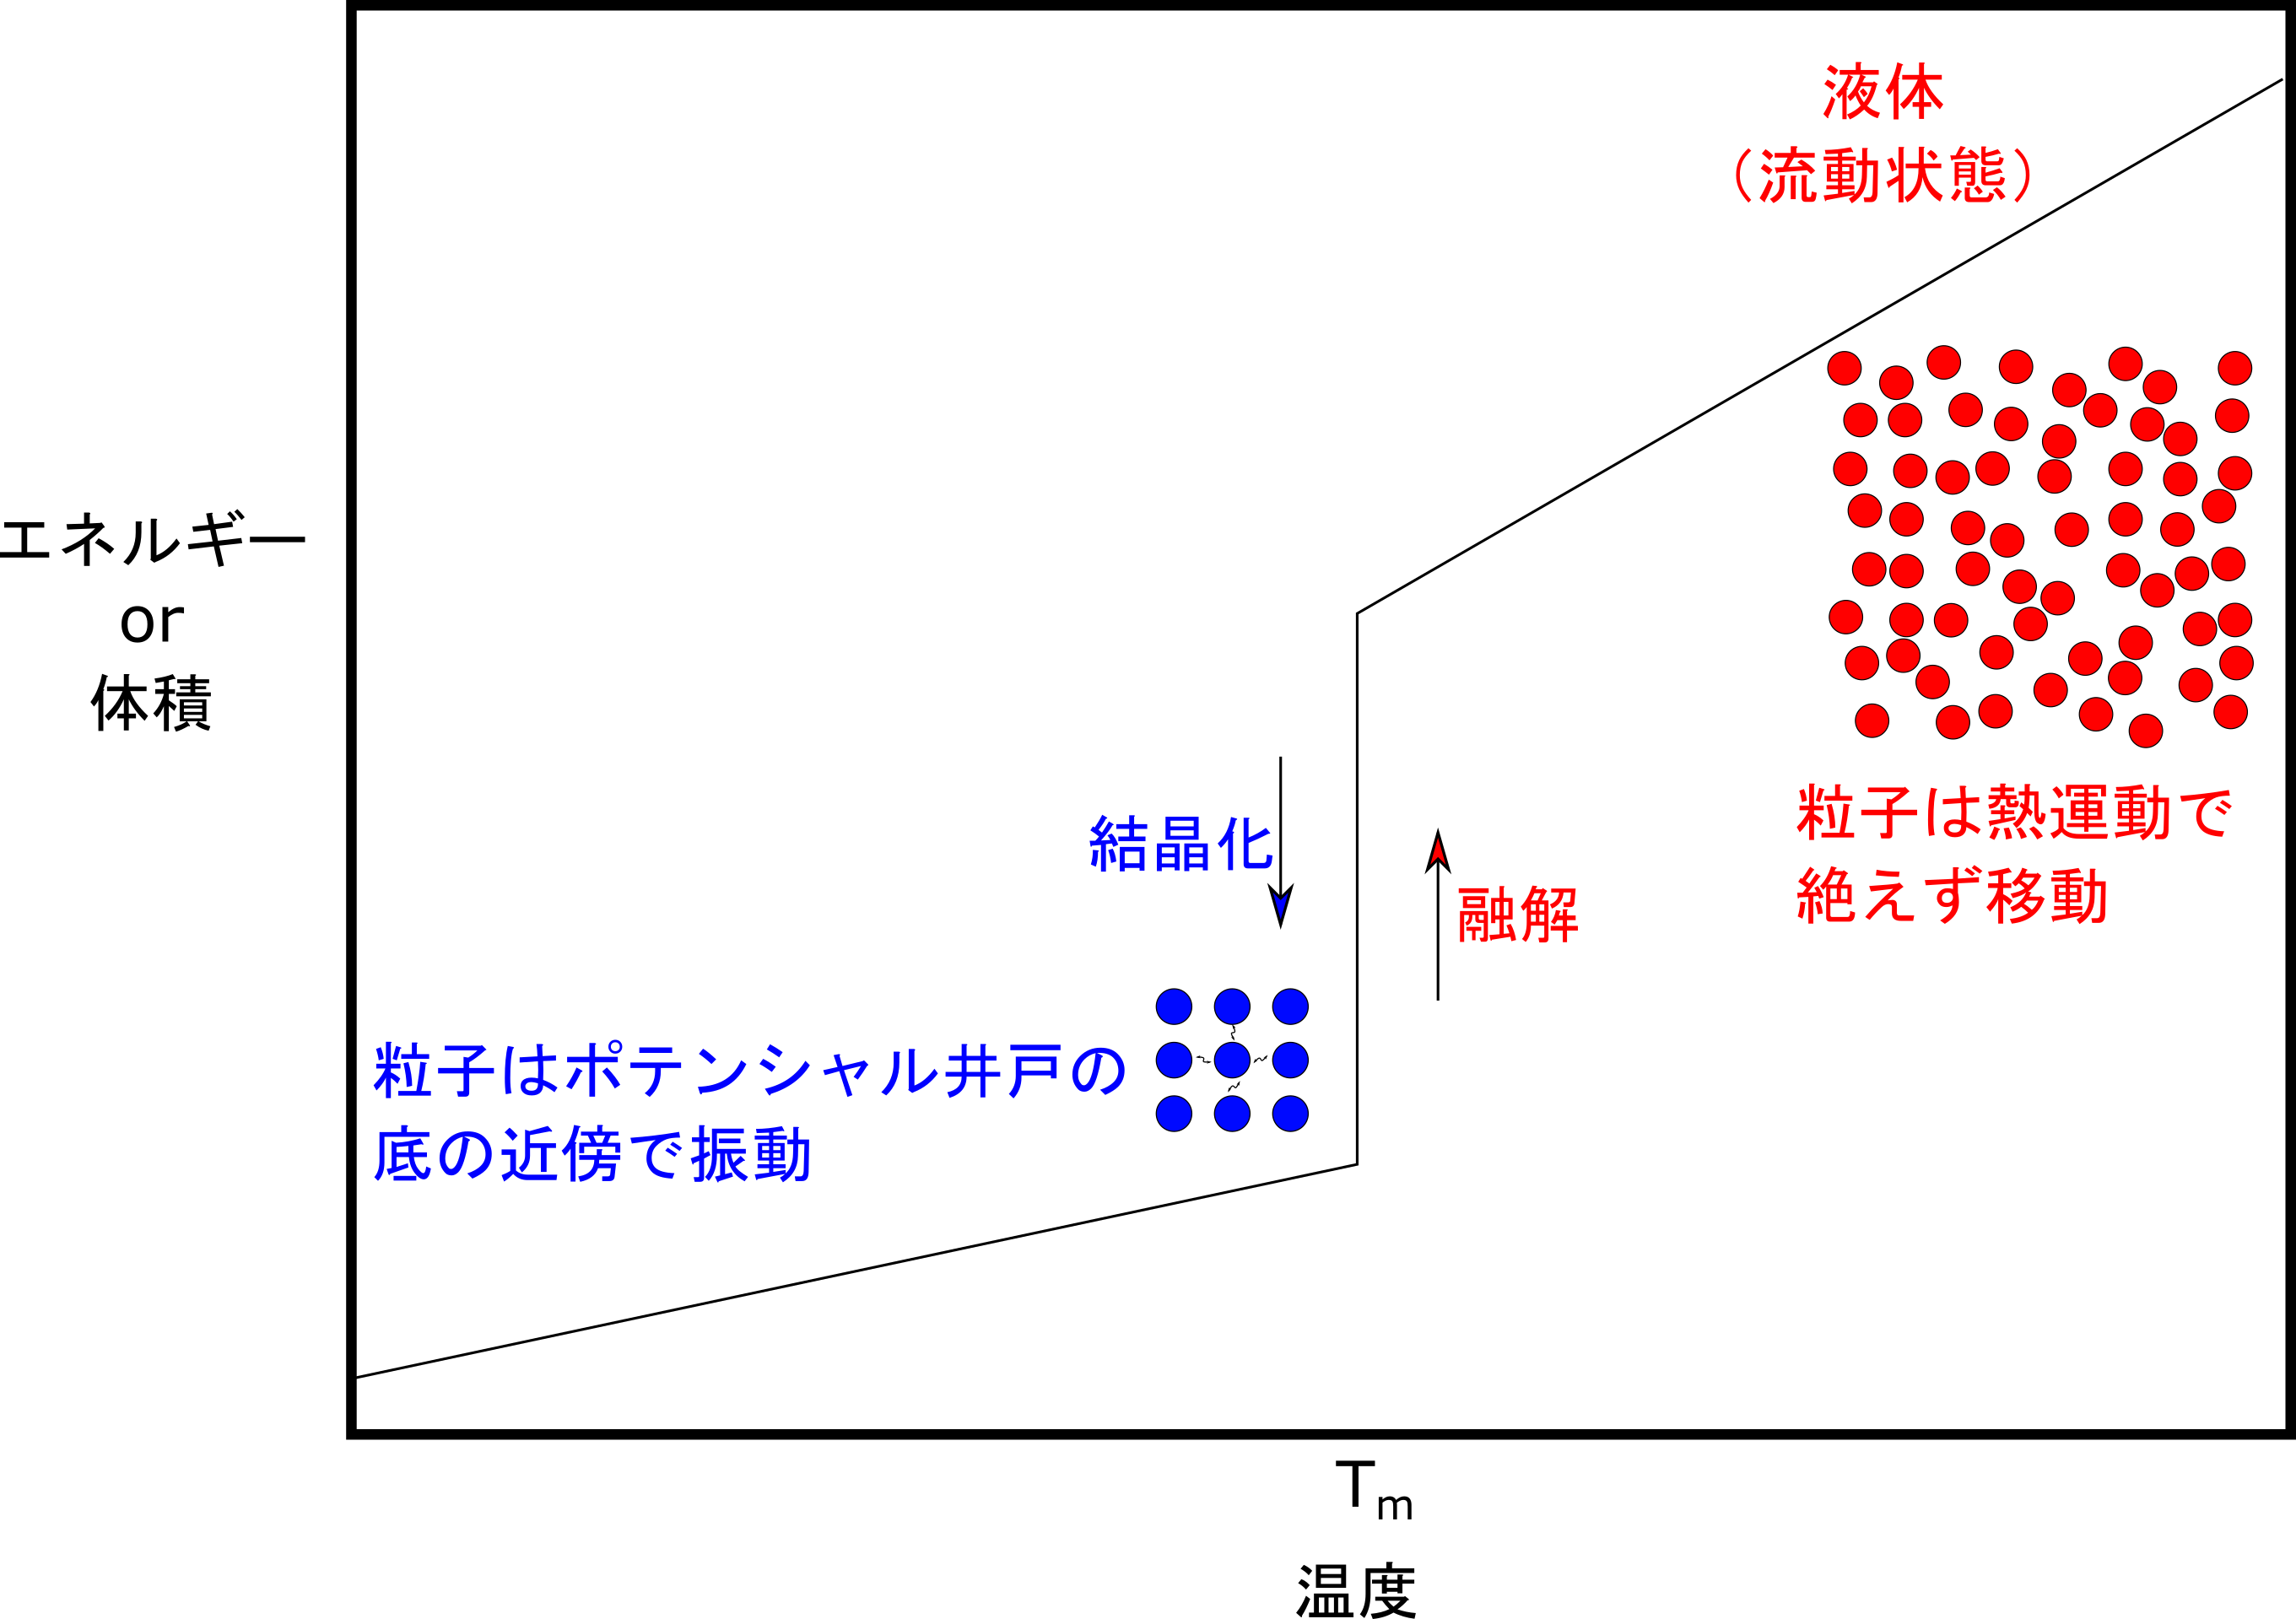
\includegraphics[width=.8\textwidth]{crystal_melt.png}
		\end{center}
\end{frame}

\section{流れるということは?}

\subsection{マクロな変形と粒子の移動}
\begin{frame}
	\frametitle{流れるということ}
	\begin{alertblock}{流れるということは}
		\begin{itemize}
			\item マクロな変形を与える。
			\begin{itemize}
				\item ミクロに見れば、粒子の相互位置が変わる。
				\item 相互のポテンシャルのために居心地が悪い粒子が発生。
				\item その結果として、粒子の移動のバランスが変化。
				% \item 「密度の揺らぎによる隙間」への粒子の移動。
				\item 結果として、居心地のいい位置へと粒子が再配置。
			\end{itemize}
			\item マクロな変形に応じて、粒子の位置が最適化。
		\end{itemize}
	\end{alertblock}
	\begin{exampleblock}{ミクロな流動のイメージ}
		\begin{columns}[T, onlytextwidth]
			\column{.7\linewidth}
			\begin{itemize}
				\item それぞれの粒子の移動の方向が、\\一方向に優先
				\item 結果として、マクロな変形に従う\\ように再配置。
			\end{itemize}
			\column{.28\linewidth}
			\begin{center}
				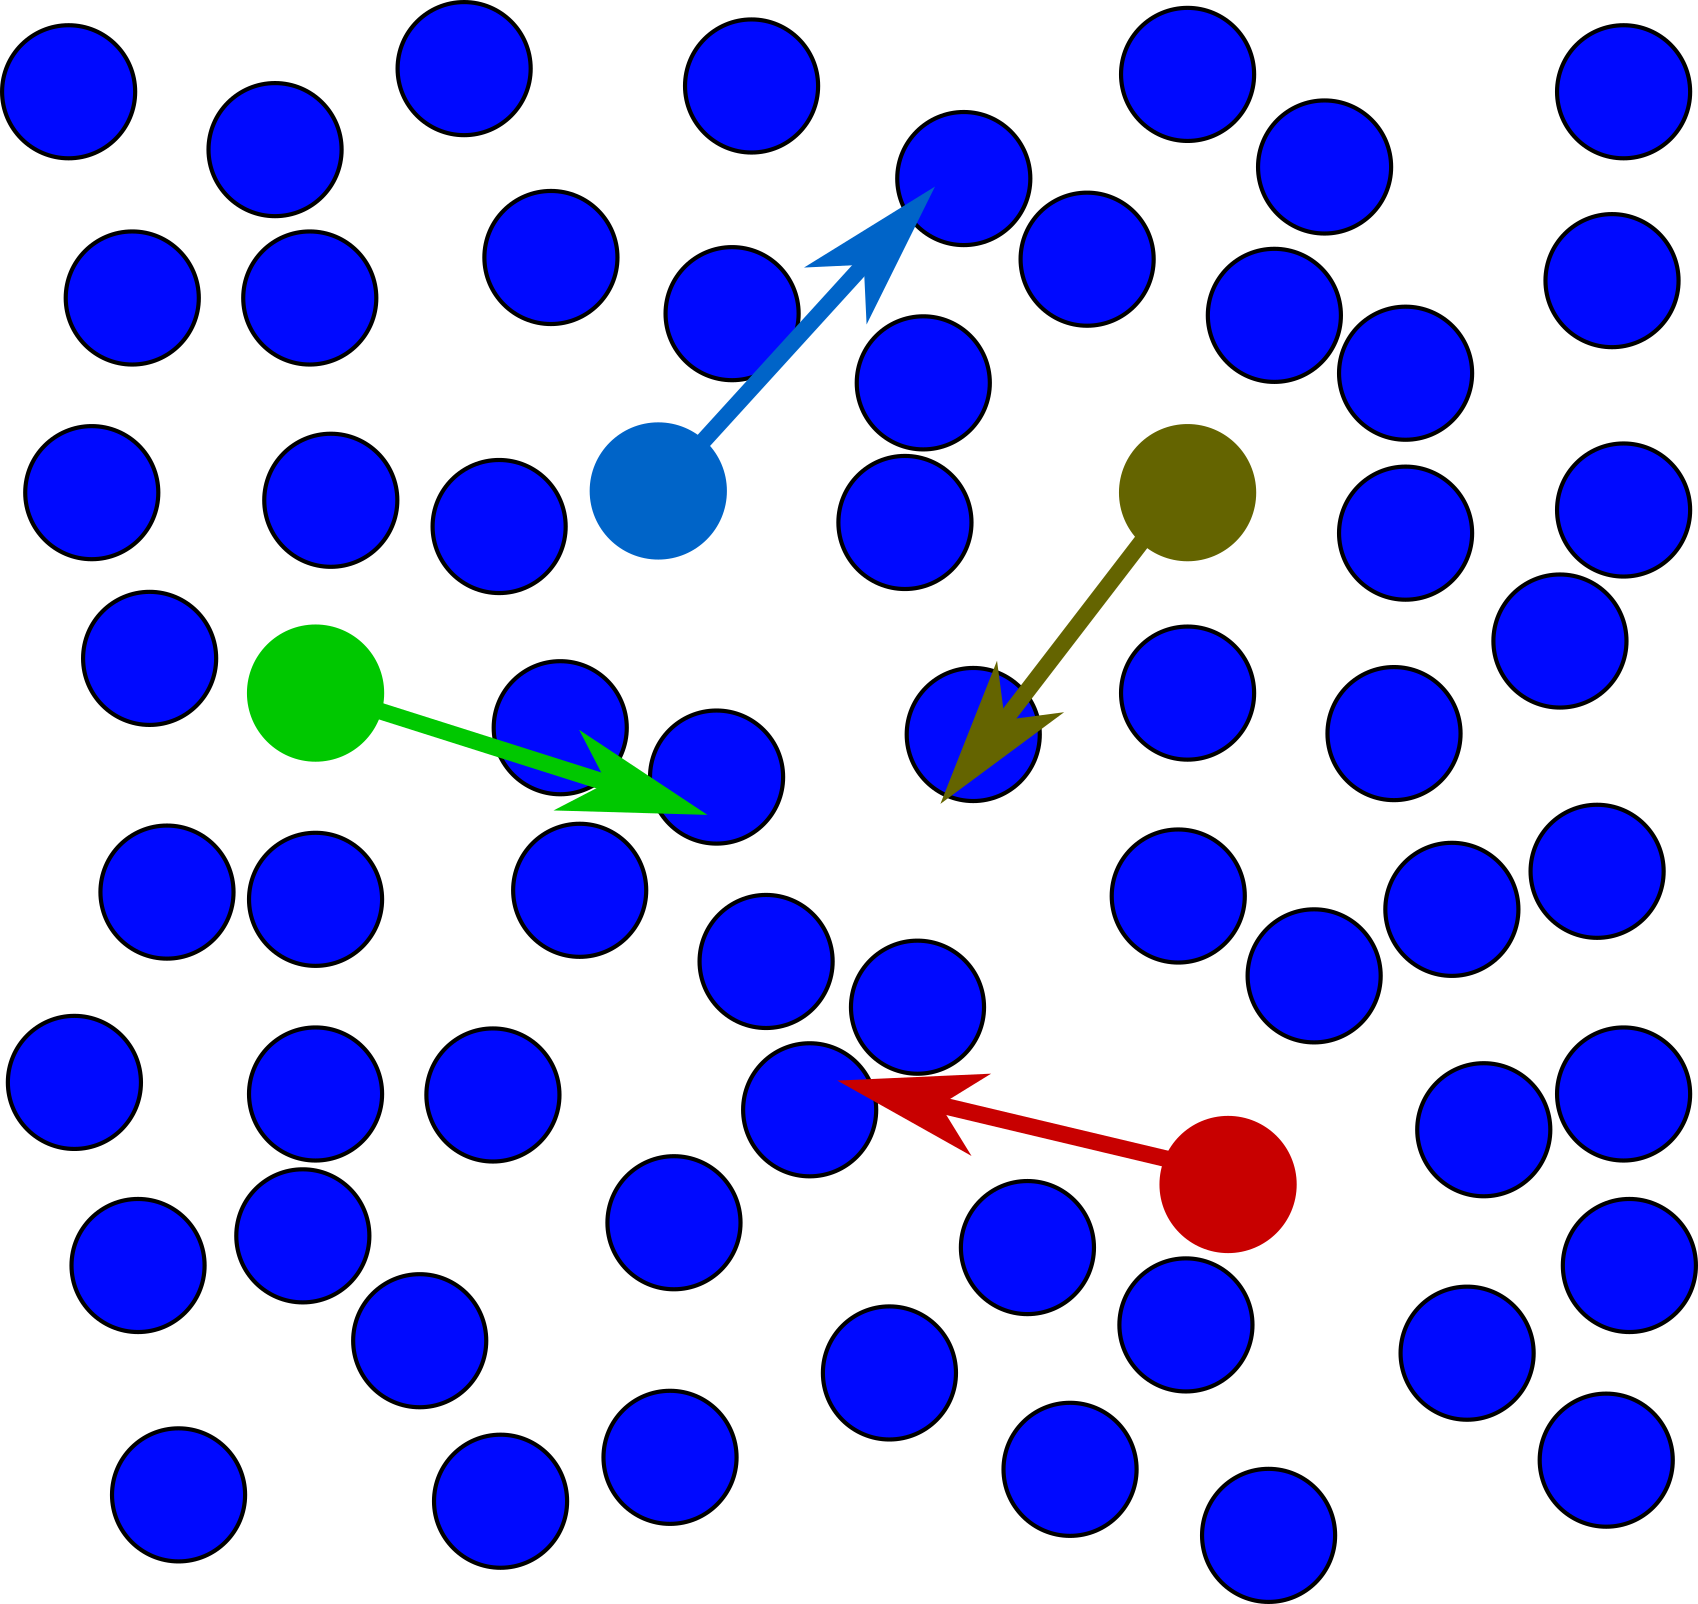
\includegraphics[width=.6\textwidth]{liquid_model_2.png}
			\end{center}
		\end{columns}
	\end{exampleblock}
\end{frame}

\begin{frame}
	\frametitle{液体の空隙と粒子の移動}
		\begin{columns}[T, onlytextwidth]
			\column{.48\linewidth}
				\begin{itemize}
					\item 液体の相互の位置は、規則的ではない。
					\item 粒子径(r/σ=1)より少し離れた所にピーク。
					\item それより少し遠くに、密度の低い領域が。
				\end{itemize}
					\begin{center}
						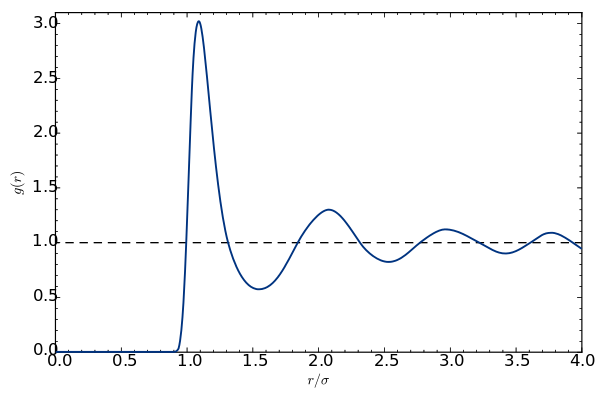
\includegraphics[width=\textwidth]{gr_2.png}
					\end{center}
			\column{.48\linewidth}
				\begin{exampleblock}{液体での粒子の移動}
					\begin{itemize}
						\item 乱雑に並んだ粒子が\\それぞれ運動。
						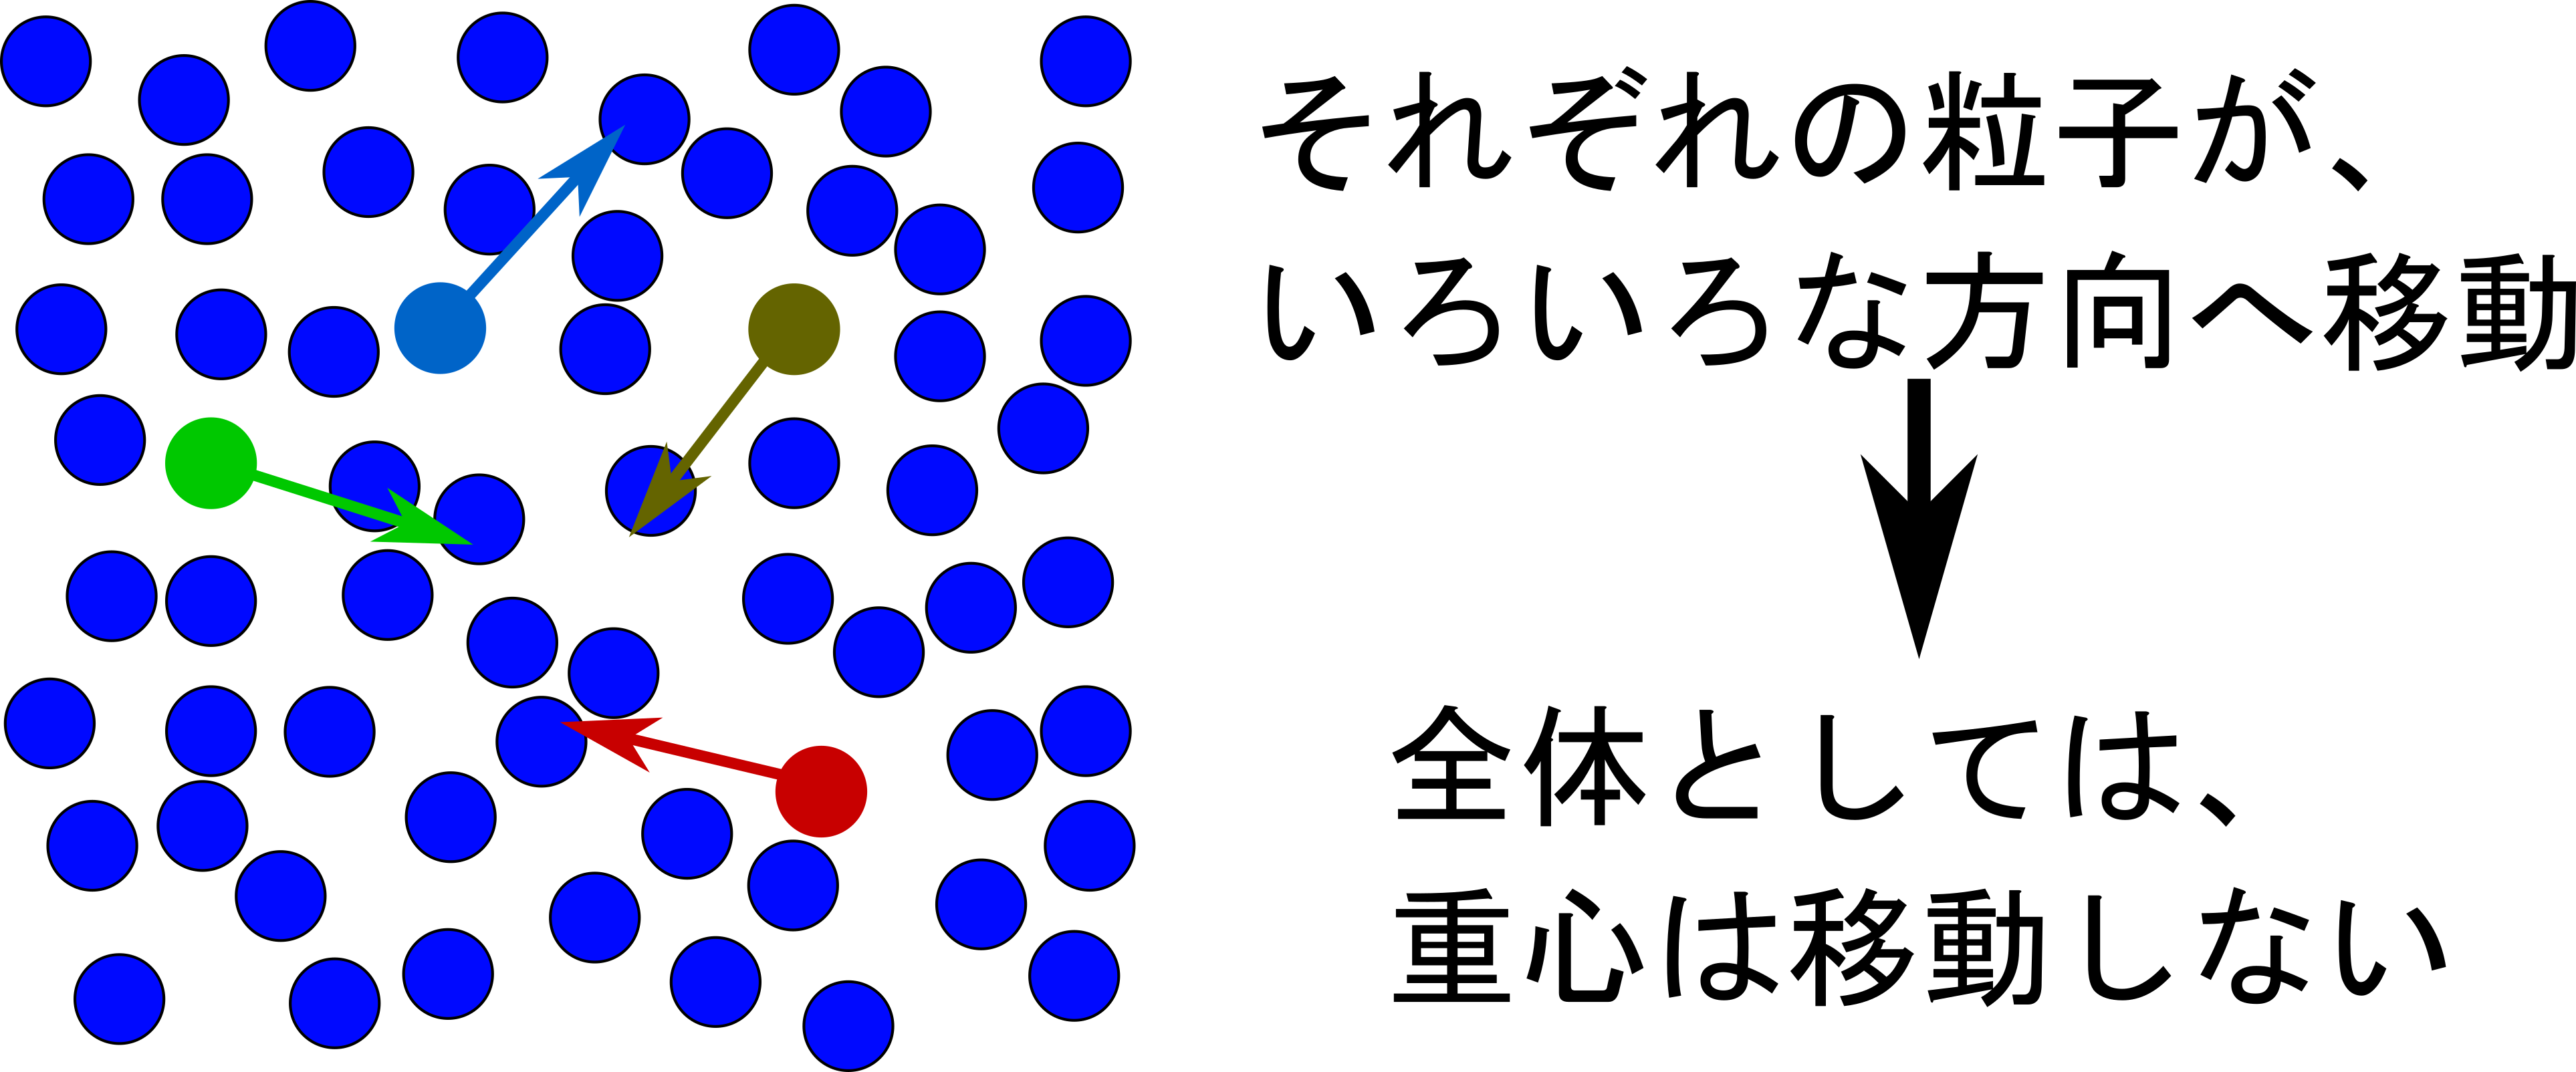
\includegraphics[width=.85\textwidth]{liquid_model.png}
						\item 一粒子に着目すると、少しずつ元の位置から移動
						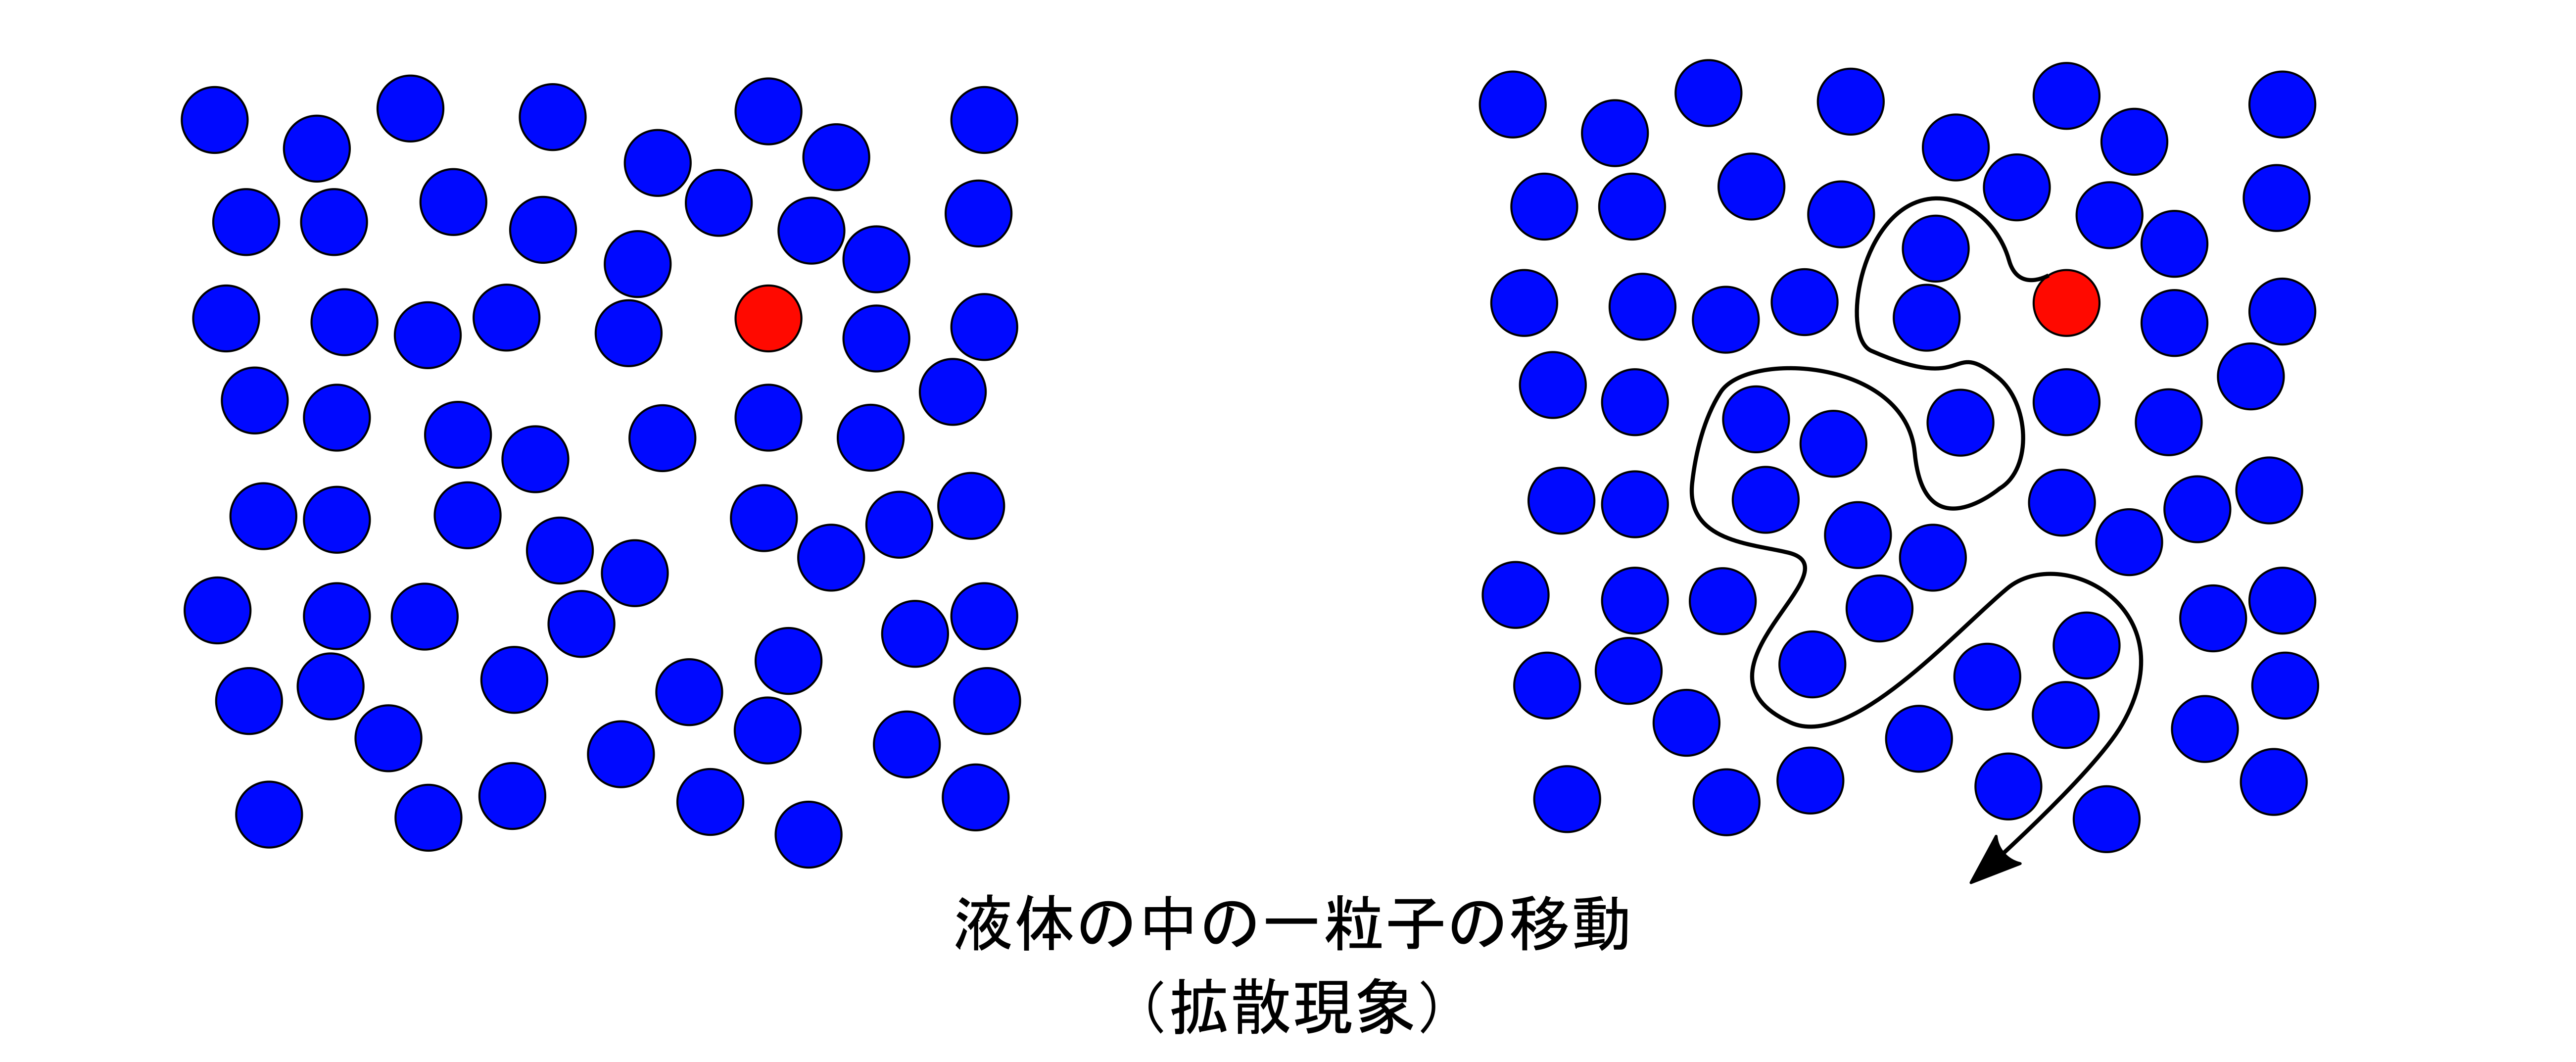
\includegraphics[width=.85\textwidth]{liquid_1.png}
					\end{itemize}
				\end{exampleblock}
		\end{columns}
\end{frame}

\subsection{固体と液体の境目は?}
\begin{frame}
	\frametitle{固体と液体の境目は?}
	\vspace{-5mm}
	\begin{columns}[T, onlytextwidth]
		\column{.48\linewidth}
			\begin{alertblock}{速い変形では固体的に}
				\begin{itemize}
					\item 流動するとは、
					\begin{itemize}
						\item 隙間に粒子が移動
						\item 空いた場所に他の粒子が移動
					\end{itemize}
					\item 粒子が動くより早く変形しようとすると?
					\begin{itemize}
						\item 速い速度で水を変形\\(高所から飛び込み)
						\item 液体が固体的な挙動
					\end{itemize}
				\end{itemize}
				\vspace{-3mm}
					\begin{center}
						
\includegraphics[width=.4\textwidth]{dive.png}
					\end{center}
			\end{alertblock}
		\column{.48\linewidth}
			\begin{exampleblock}{長時間では液体的に}
				\begin{center}
					長時間では氷河も流れる。
					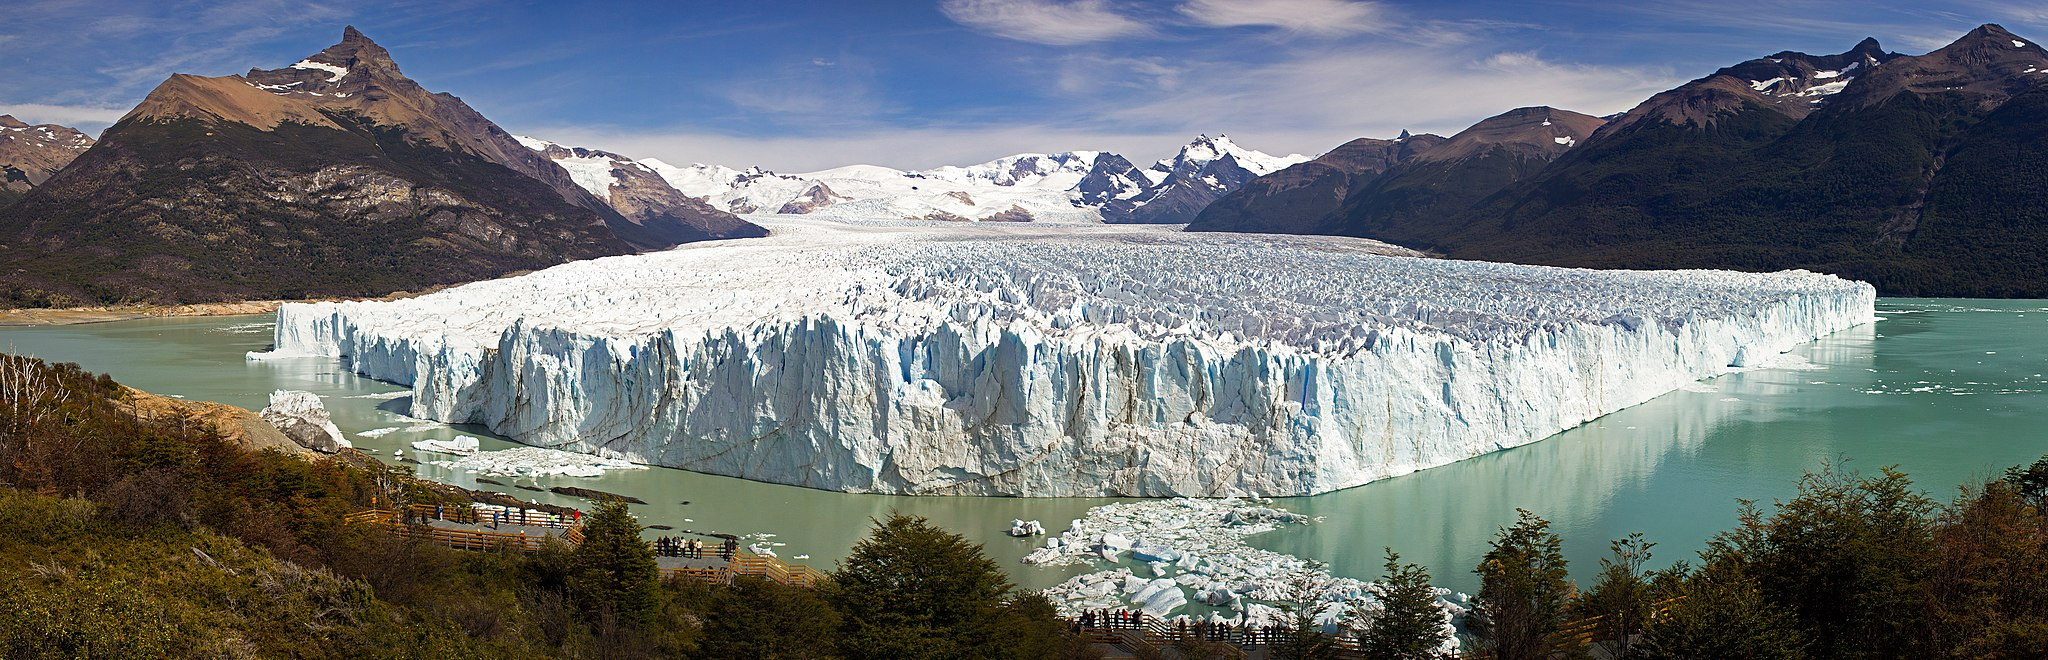
\includegraphics[width=\textwidth]{hyoga.jpg}
					% \vspace{5mm}
					コールタールも
					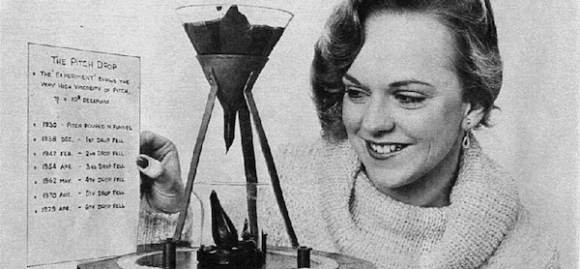
\includegraphics[width=\textwidth]{pitchdrop.png}

					\href{https://livestream.com/accounts/4931571/events/5369913}{\textcolor{blue}{ピッチドロップ実験の\\ライブ画像へのリンク}}
				\end{center}
			\end{exampleblock}
	\end{columns}	
\end{frame}

\subsection{ガラス状態}
\begin{frame}
	\frametitle{結晶と非晶(ガラス状態)}
	\begin{columns}[T, onlytextwidth]
		\column{.48\linewidth}
			\begin{itemize}
				\item 液体からの冷却で、
				\item 常に結晶化するとは限らない。
				\begin{itemize}
					\item 非晶体:アモルファス
					\item 流れない
					\item 例えば、窓ガラス等
				\end{itemize}
			\end{itemize}
			\begin{center}
				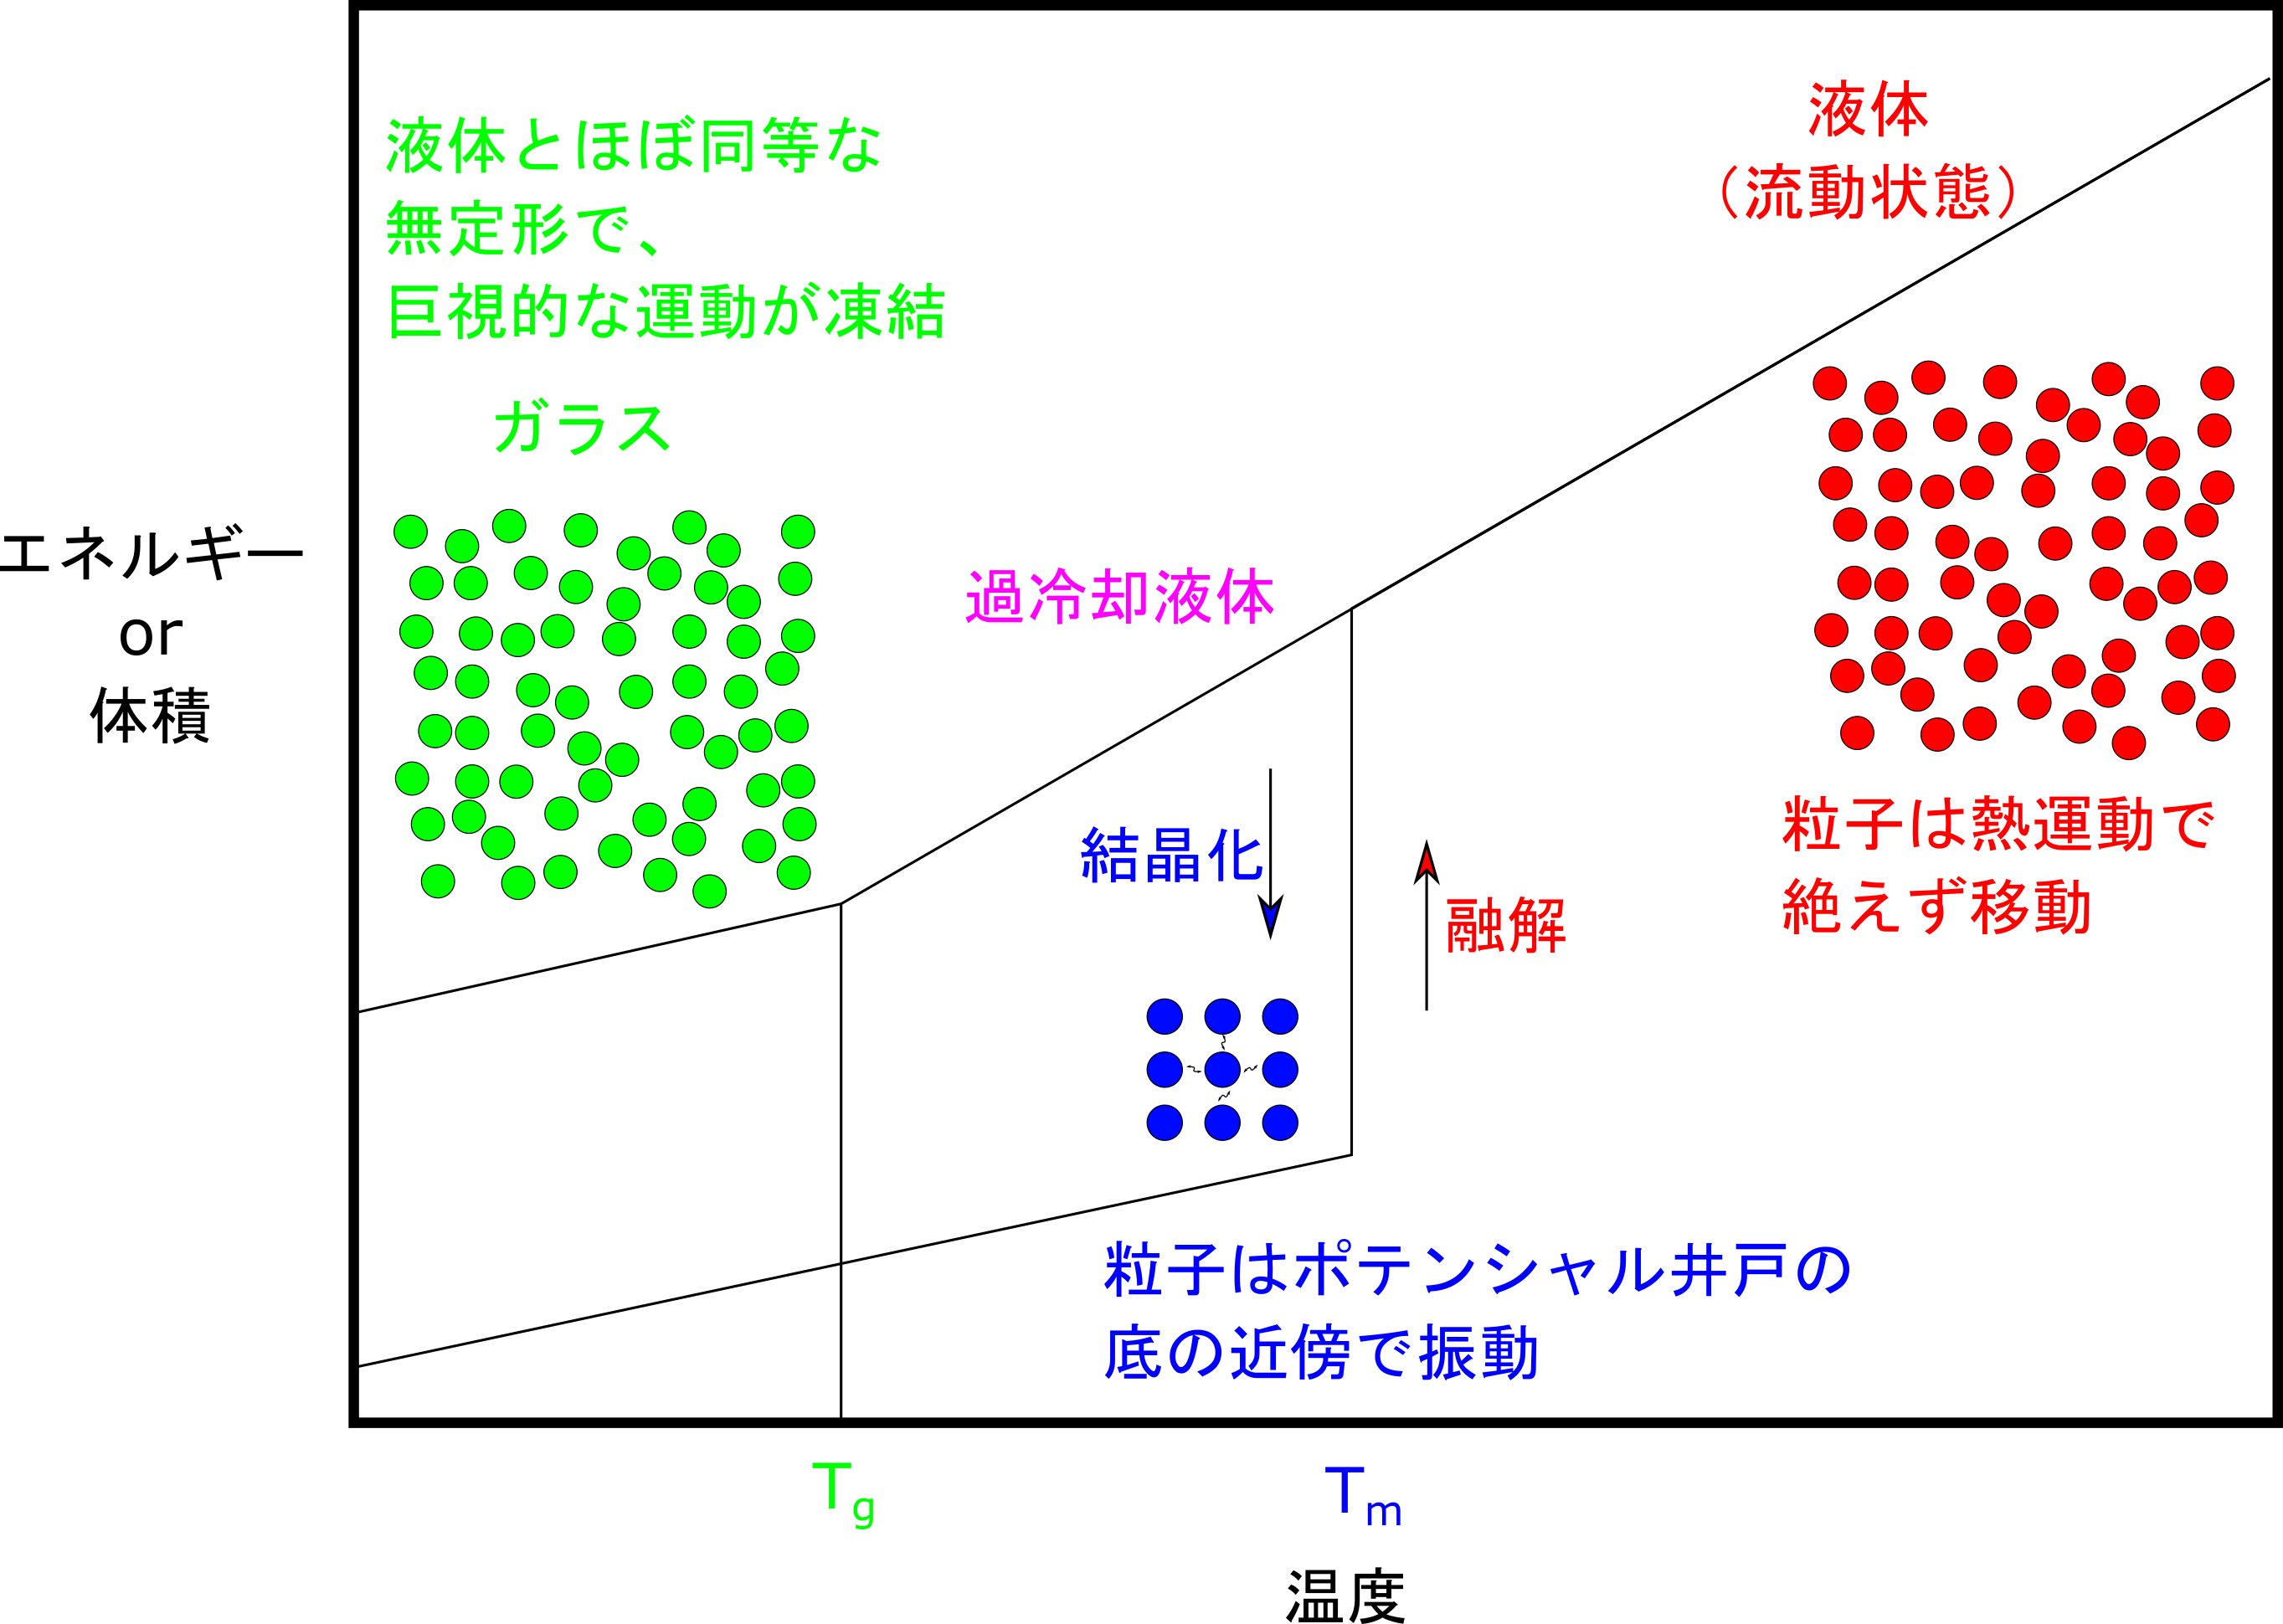
\includegraphics[width=.9\textwidth]{glass_trans.png}
			\end{center}
		\column{.48\linewidth}
			\begin{itemize}
				\item 単純な粒子であれば並びやすい(下図の左下)
				\item 複雑な形状では、非晶でもそれほど不安定ではない。
			\end{itemize}
			\begin{center}
				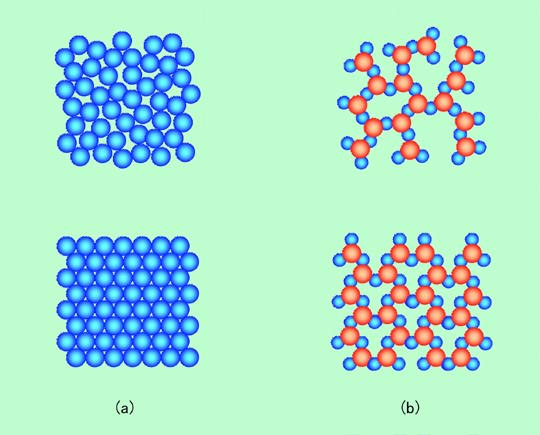
\includegraphics[width=.8\textwidth]{glass_1.jpg}

				\href{https://hr-inoue.net/zscience/topics/glass/glass.html}{\small{この絵のサイトへのリンク}}
			\end{center}
	\end{columns}
\end{frame}

\begin{frame}
	\frametitle{ポリマー(N=2)のガラス状態}
		\begin{columns}[T, onlytextwidth]
			\column{.48\linewidth}
				\begin{itemize}
					\item ポリマーの多くは、非晶性でガラス化。
					\begin{itemize}
						\item 多数の粒子がつながるため結晶化が抑制。
						\item 容易にガラス化
					\end{itemize}
				\end{itemize}	
				\begin{center}
					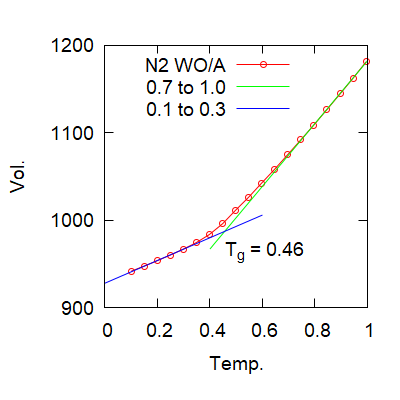
\includegraphics[width=.85\textwidth]{N2_NoAng_NV_T.png}

					\scriptsize{体積変化のシミュレーション}
				\end{center}
			\column{.48\linewidth}
			\textcolor{blue}{N=2 の最小ポリマーモデル}
				\begin{itemize}
					\item 液体状態 T=1.0
					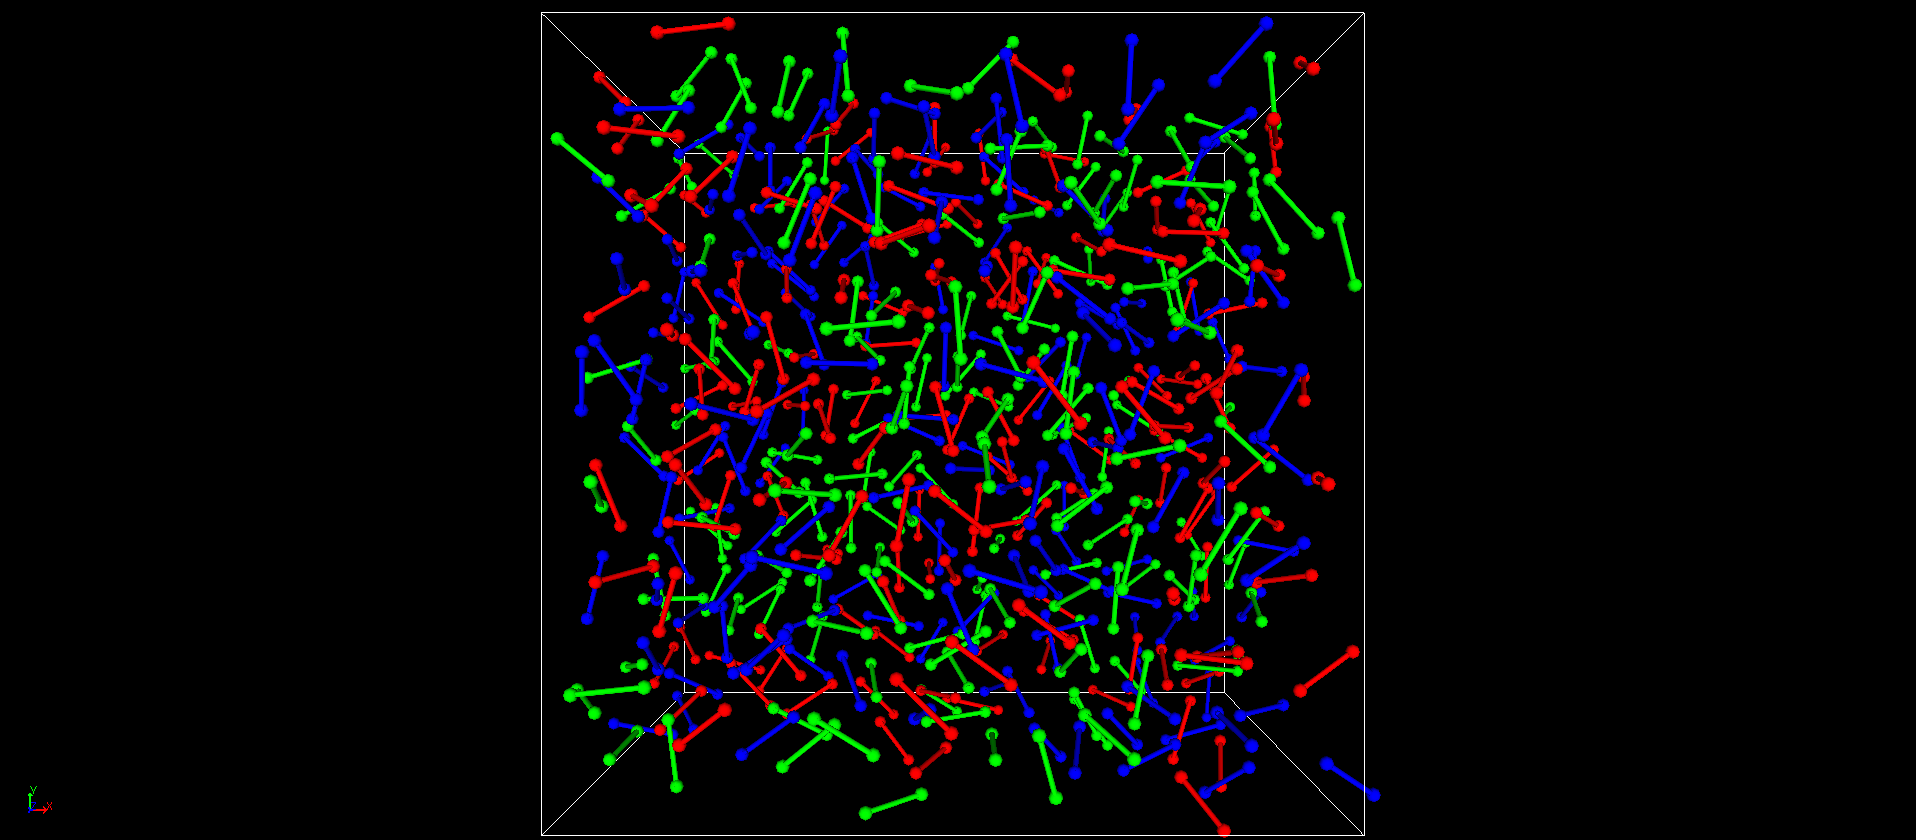
\includegraphics[width=.9\textwidth]{N2_T_1.png}
					\href{https://drive.google.com/file/d/1V5lLeoqhoUcujVnHqEzFumDlGXC_rPe-/view?usp=sharing}{動画へのリンク}
					\item ガラス状態 T=0.1
					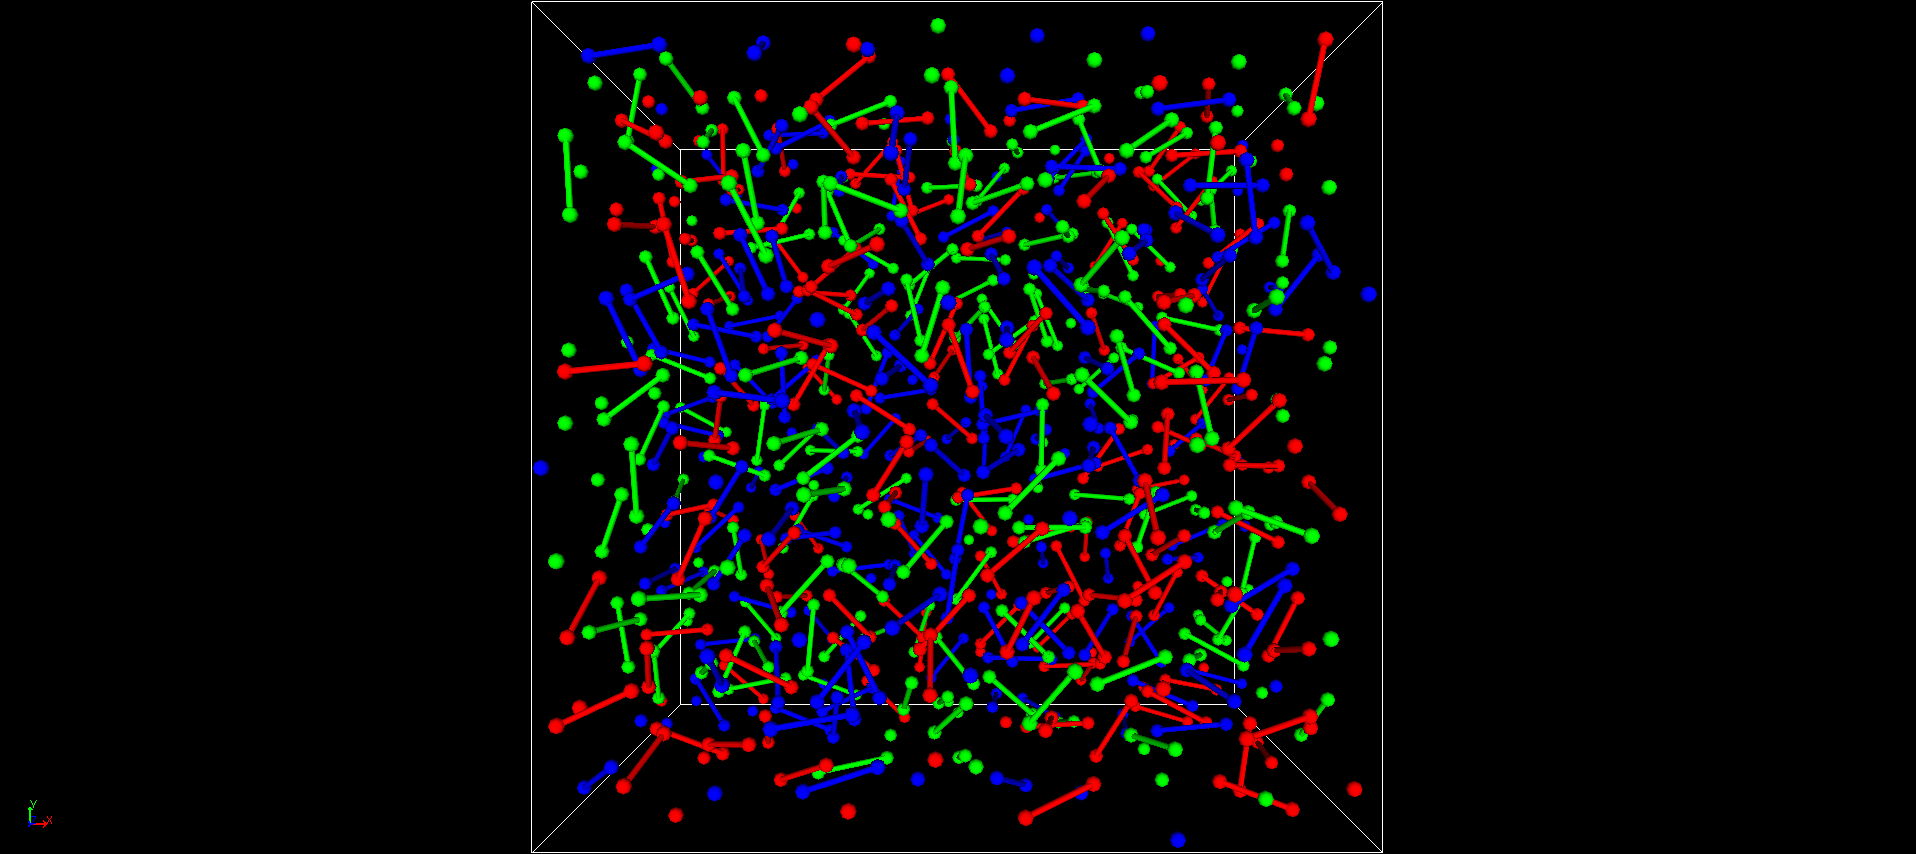
\includegraphics[width=.9\textwidth]{N2_T_0_1.png}
					\href{https://drive.google.com/file/d/1HBZ6eQQp0o2vft4bUGxRJUwv4vabs_7d/view?usp=sharing}{動画へのリンク}
				\end{itemize}
		\end{columns}
\end{frame}

\section{応力の由来は?}
\subsection{物質の変形と応力}
\begin{frame}
	\frametitle{物質の変形と応力}
		\begin{columns}[T, onlytextwidth]
			\column{.44\linewidth}
				\begin{block}{物質を変形させると?}
					\begin{itemize}
						\item 変形を単純化すると
						\begin{itemize}
							\item 引張変形
							\item ずり変形
						\end{itemize}
						\item 変形により、
						\begin{itemize}
							\item 物質は歪んで、
							\item 内部で応力が発生
						\end{itemize}
					\end{itemize}
				\end{block}
				\begin{center}
					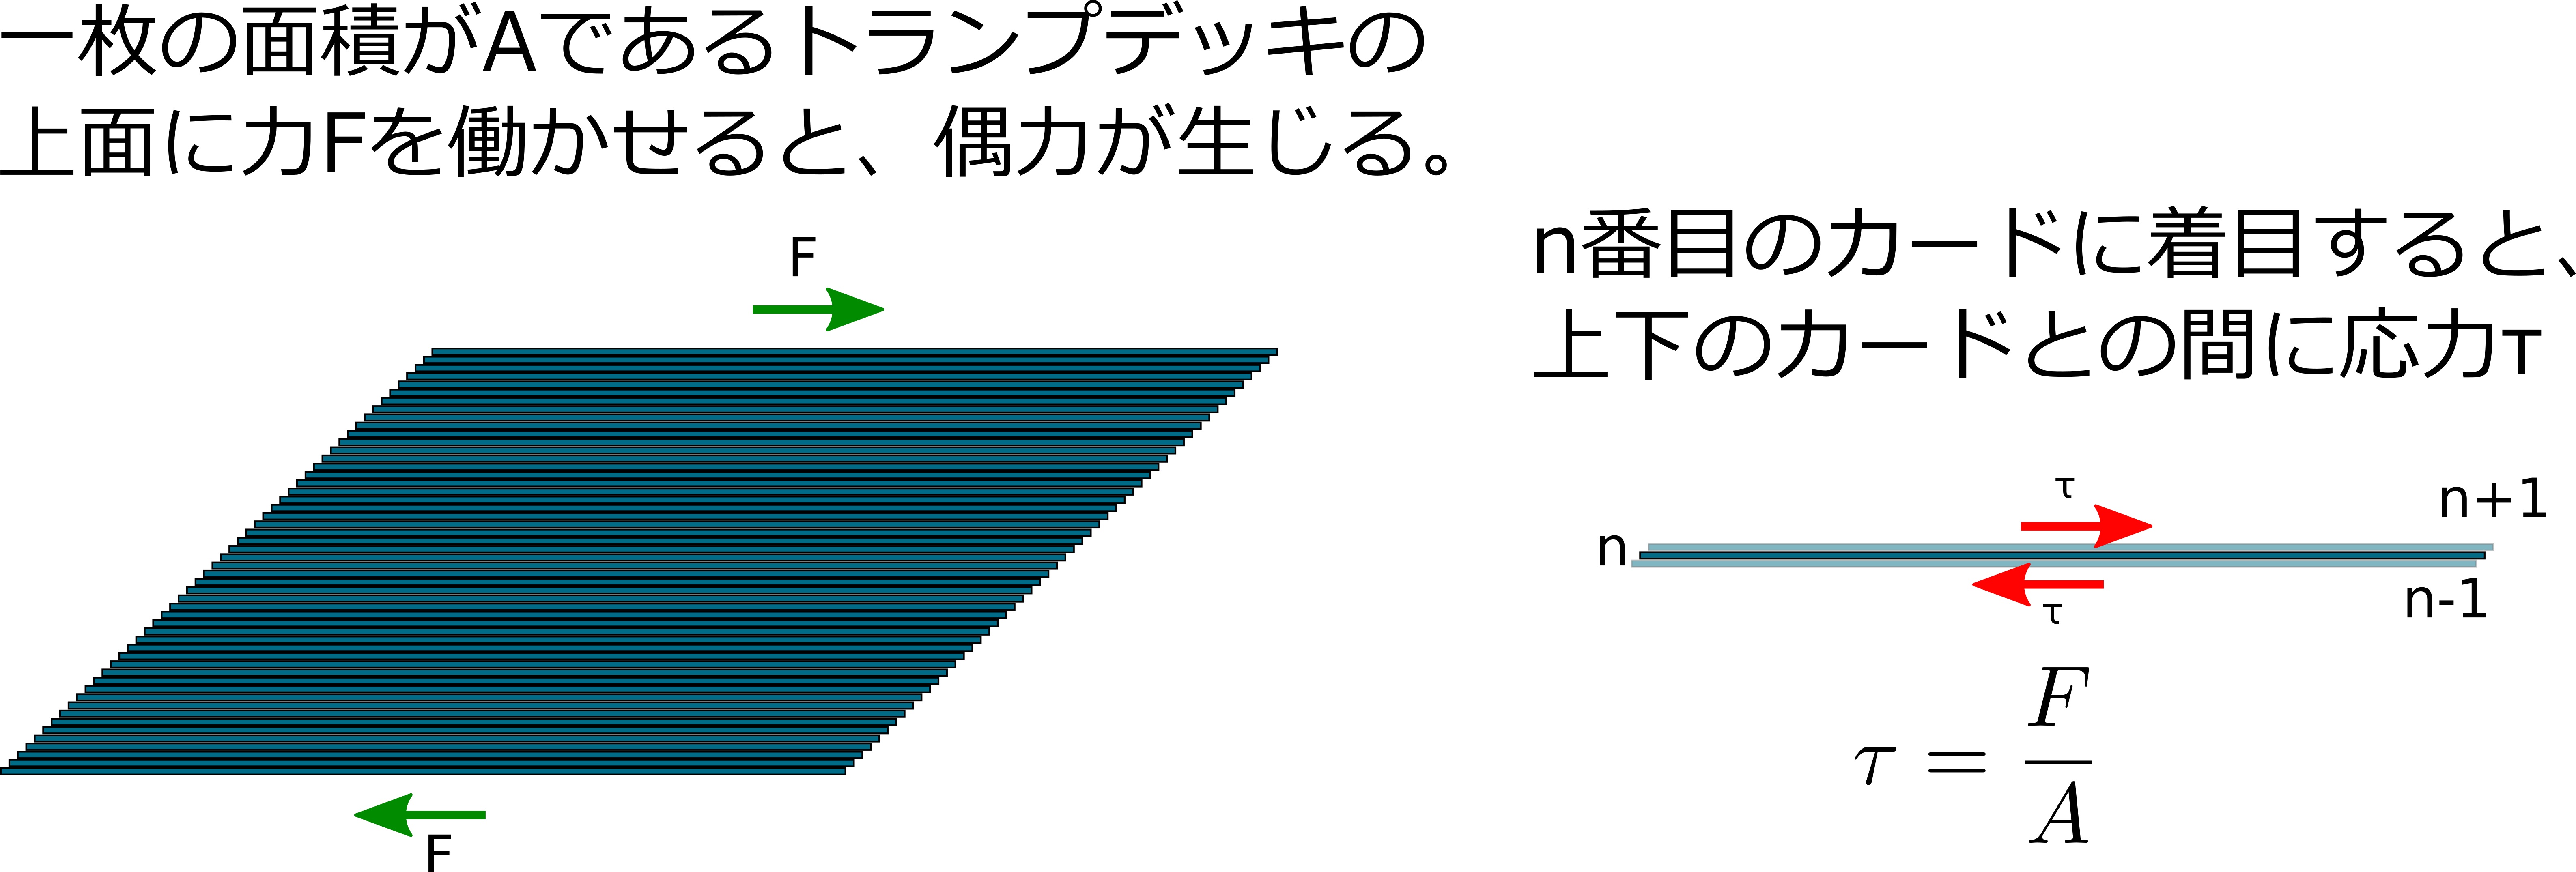
\includegraphics[width=\textwidth]{trump_deck.png}
				\end{center}
			\column{.52\linewidth}
				\begin{exampleblock}{固体と液体の違い}
					\begin{itemize}
						\item 固体では
						\begin{itemize}
							\item 単純な固体は一様に\\変形
							\item 生じる応力が一様
						\end{itemize}
						\item 液体の場合
						\begin{itemize}
							\item 変形を止めれば、\\応力も消失
							\item 液体内部での変形
							\begin{itemize}
								\item 粒子同士の相互作用が増加
								\item 粒子が移動すれば、増加分が消失
							\end{itemize}
						\end{itemize}
					\end{itemize}
				\end{exampleblock}
		\end{columns}
\end{frame}

\begin{frame}
	\frametitle{物質の変形と応力}
		\begin{columns}[T, onlytextwidth]
			\column{.44\linewidth}
				\begin{block}{物質を変形させると?}
					\begin{itemize}
						\item 変形を単純化すると
						\begin{itemize}
							\item 引張変形
							\item ずり変形
						\end{itemize}
						\item 変形により、
						\begin{itemize}
							\item 物質は歪んで、
							\item 内部で応力が発生
						\end{itemize}
					\end{itemize}
				\end{block}
				\begin{center}
					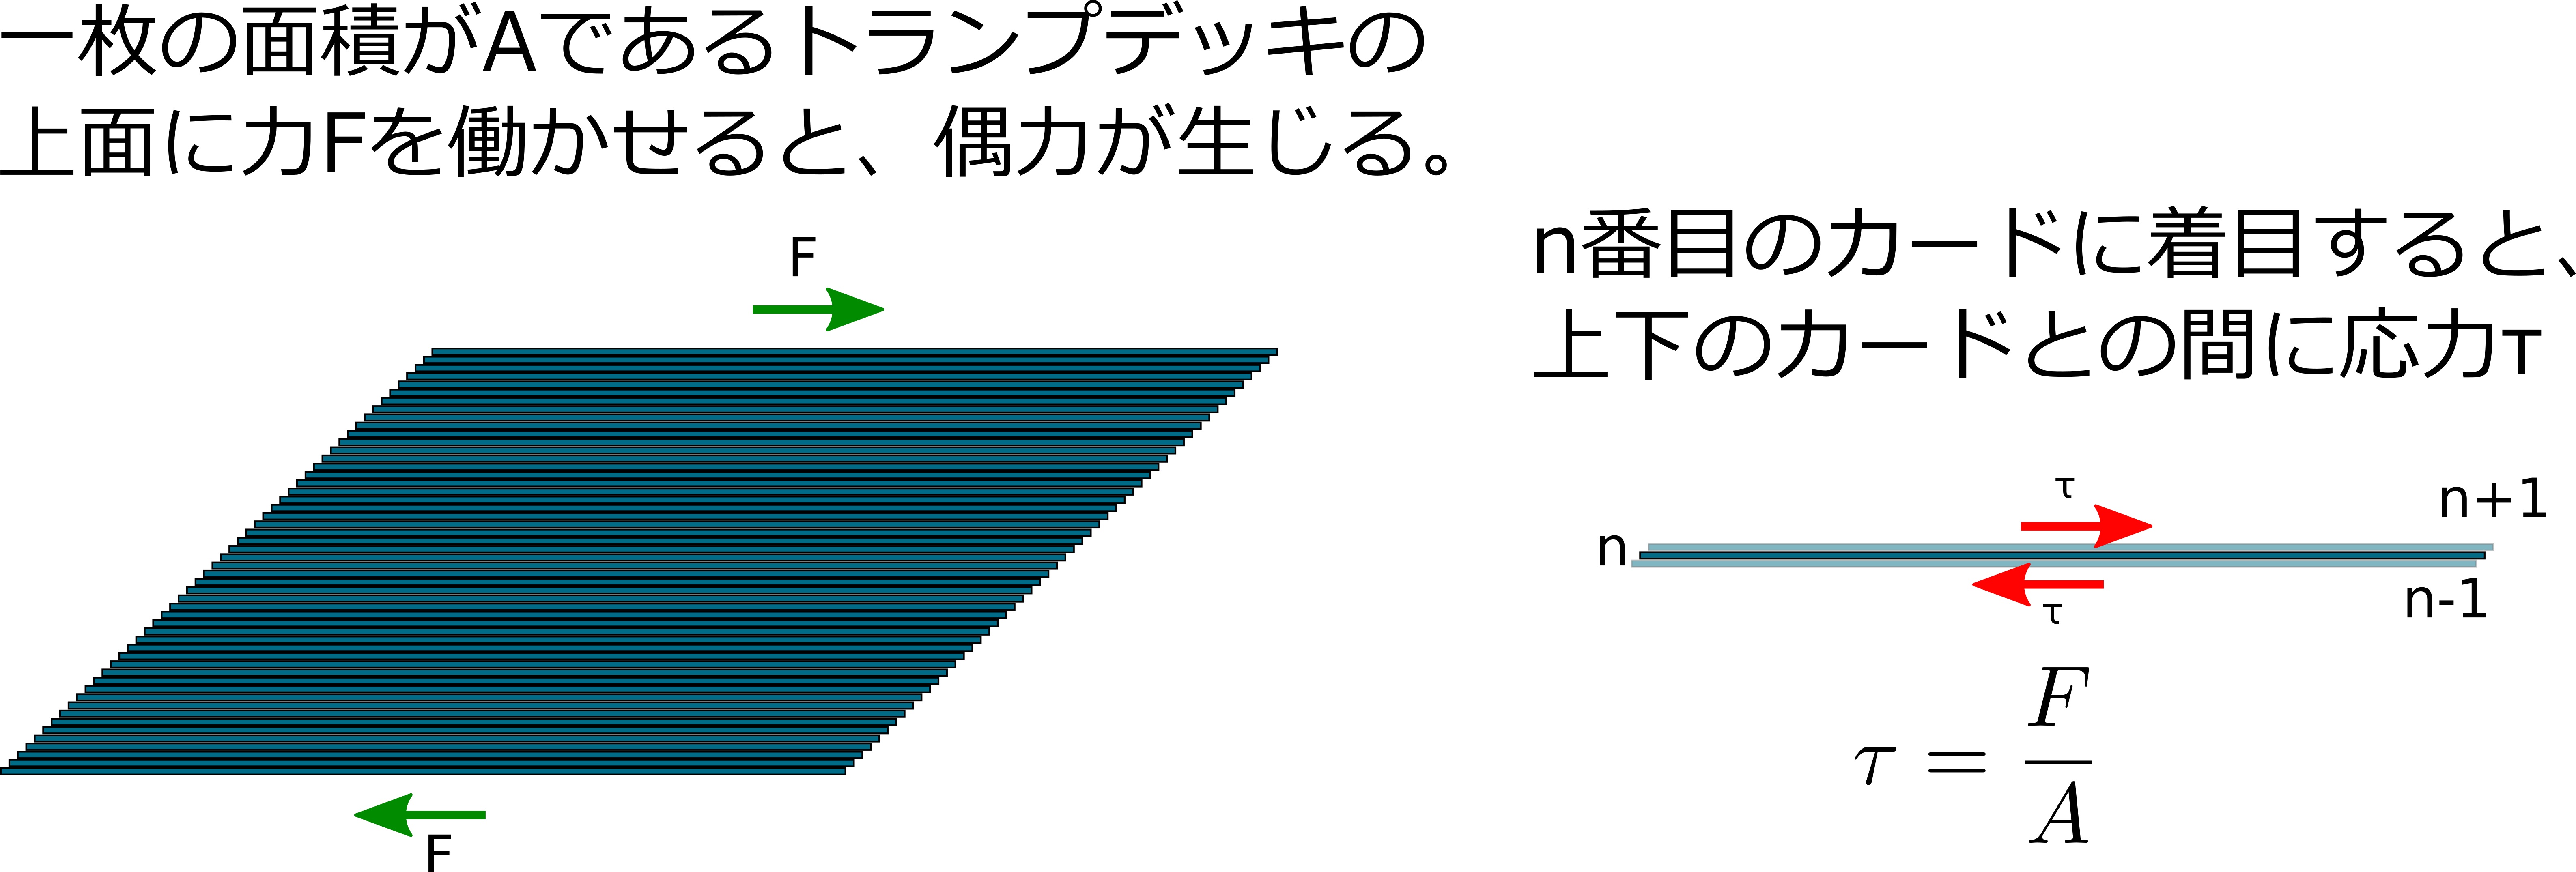
\includegraphics[width=\textwidth]{trump_deck.png}
				\end{center}
			\column{.52\linewidth}
				\begin{exampleblock}{注意点}
					\begin{itemize}
						\item ここでの変形は、
						\begin{itemize}
							\item 線形応答となるような\alert{微小な変形}を考える。
							\item その時の系の応答である応力は、
							\item \alert{重ね合わせの適応できる理想的}なものとなる。
						\end{itemize}
						\item そのような\alert{応力の起源}を考えよう。
					\end{itemize}
				\end{exampleblock}
		\end{columns}
\end{frame}

\subsection{結晶の応力の起源}
\begin{frame}
	\frametitle{結晶の応力の起源}
		\vspace{-3mm}
		\begin{columns}[T, onlytextwidth]
			\column{.48\linewidth}
				\begin{exampleblock}{マクロな変形を付与}
						\begin{itemize}
							\item 固体内部でもミクロに変形
							\item マクロと相似にミクロな変形と単純化
							\item 粒子間で安定位置から変位
						\end{itemize}
				\end{exampleblock}
				\begin{center}
					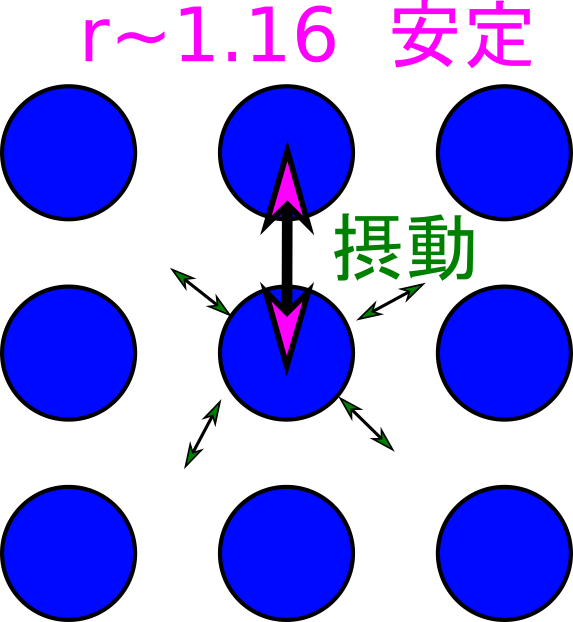
\includegraphics[width=.45\textwidth]{LJ_ryusi.png}
				\end{center}
			\column{.48\linewidth}
				\begin{block}{ミクロに安定位置から変位}
					\begin{itemize}
						\item 局所的には二体間で、
						\begin{itemize}
							\item 接近 $\Leftrightarrow$ 斥力
							\item 離反 $\Leftrightarrow$ 引力
						\end{itemize}
						% \item その積分値として、\\マクロな応力が発生
					\end{itemize}
				\end{block}
				\begin{center}
					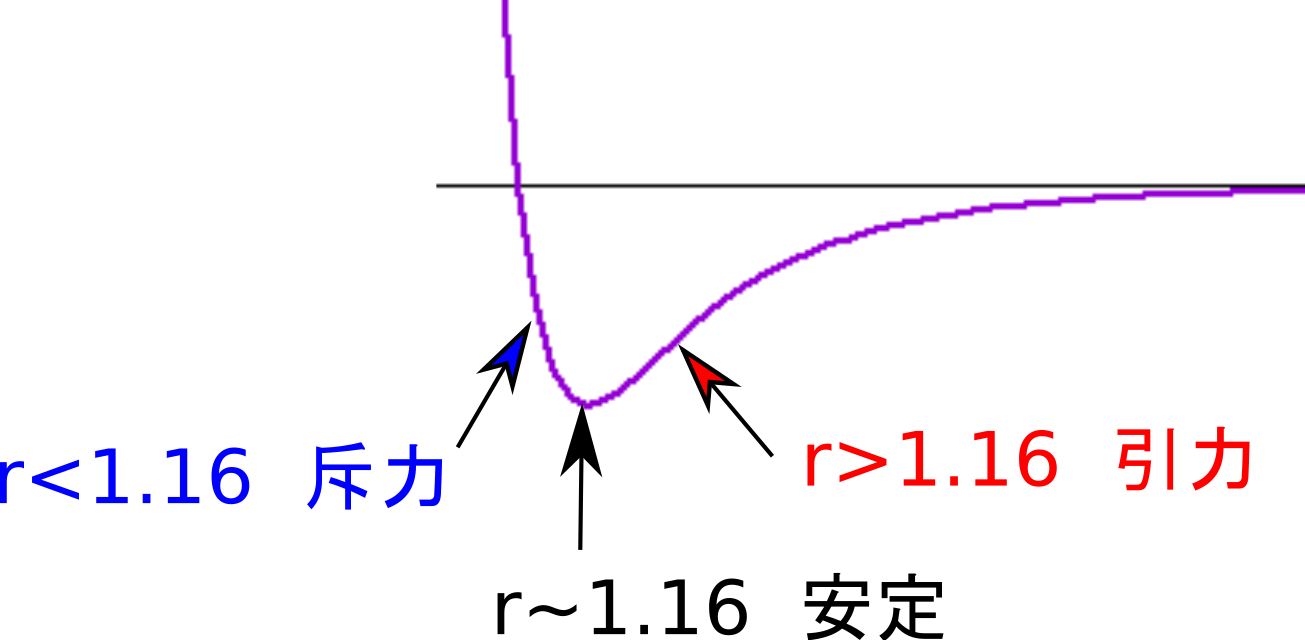
\includegraphics[width=.8\textwidth]{LJ_pos.png}
				\end{center}
				\begin{alertblock}{マクロな応力は}
					\begin{itemize}
						% \item 局所的には二体間で、
						% \begin{itemize}
						% 	\item 接近 $\Leftrightarrow$ 斥力
						% 	\item 離反 $\Leftrightarrow$ 引力
						% \end{itemize}
						\item ミクロな応力の積分値\\$\Rightarrow$ \alert{マクロな応力}
					\end{itemize}
				\end{alertblock}
		\end{columns}
\end{frame}

\subsection{液体の応力とは?}
\begin{frame}
	\frametitle{液体の応力とは?}
		\begin{itemize}
			\item マクロな変形(例えば、ずり変形)を付与
			\begin{itemize}
				\item ミクロにも粒子近傍が変形
			\end{itemize}
			\item 一粒子に着目すると、
			\begin{itemize}
				\item その粒子を取り巻く周りの粒子とのポテンシャル場が変化して、\textcolor{red}{「歪んだかご」のようになる。}
				\item 「歪んだかご」の中で、\textcolor{red}{居心地が悪くなる。}
				\item その結果として\textcolor{red}{局所的な応力が発現}
			\end{itemize}
			\item その積分値として、マクロな応力
			\begin{itemize}
				\item 「歪んだかご」からの\alert{脱出 $\Leftrightarrow$ ミクロな応力が消失 }
				\item マクロにも\alert{流動}
			\end{itemize}
		\end{itemize}
		\vspace{3mm}
		\begin{center}
			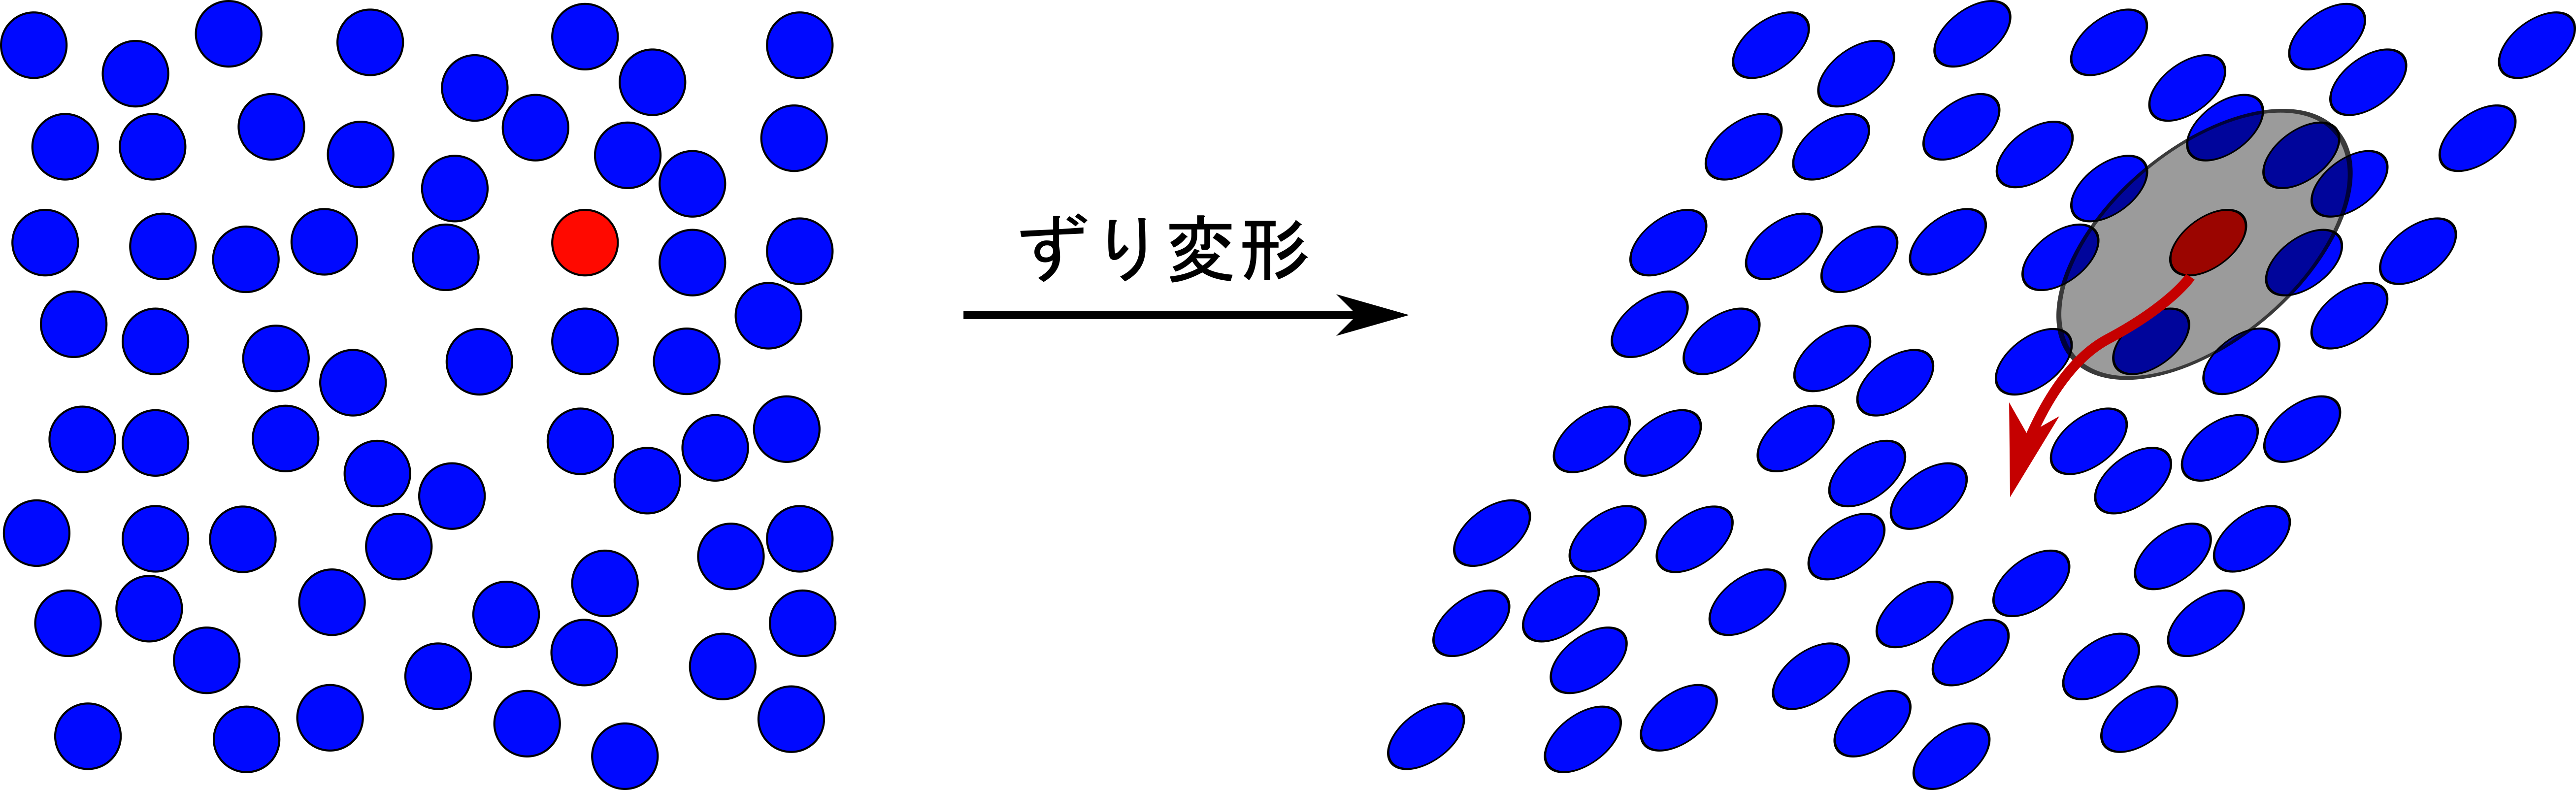
\includegraphics[width=.6\textwidth]{liquid_flow.png}
		\end{center}
\end{frame}

\begin{frame}
	\frametitle{(おまけ)猫は液体か?}
	2017 年のイグノーベル賞で、物理学賞が「猫は固体と液体両方になれるか?(Can a Cat Be Both a Solid and a Liquid?)」
		\begin{center}
			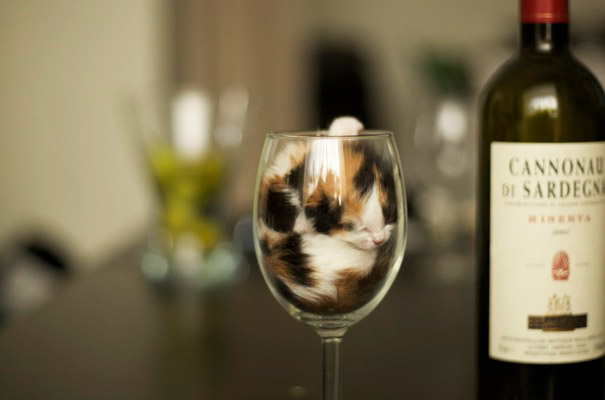
\includegraphics[width=.45\textwidth]{funny-liquid-cats-3.jpg}
		\end{center}

		ネットの画像へのリンク
		\begin{itemize}
			\item \href{https://drive.google.com/file/d/1IaglSdZWwZc_X989BEf_p33t0Ci8XHUe/view?usp=sharing}{上記論文中の猫の画像}
			\item \href{https://www.buzzfeed.com/jp/pablovaldivia/liquid-cats-1}{「ネコは液体であると証明する14枚の写真」}
			\item \href{http://karapaia.com/archives/52205481.html}{「猫の液状化」}
		\end{itemize}
\end{frame}

\begin{frame}
	\frametitle{まとめ}
	% この章では、物質の三態について物理化学的に考えてみました。
	\begin{boxnote}
		\vspace{-3mm}
		\begin{itemize}
			\item 物質の三態について
			\begin{itemize}
				\item 固体のモデルとして、規則構造の結晶を用い、
				\item 液体のモデルについては、シミュレーションも
			\end{itemize} 
			\item 流れるということは?
			\begin{itemize}
				\item マクロな変形と粒子の移動の関係のイメージ
				\item 固体と液体の境目が曖昧で、ガラス状態という中間的な状態
			\end{itemize} 
			\item 応力の由来は?
			\begin{itemize}
				\item 結晶の応力は粒子が相互に安定な状態にある
				\item 液体の応力は、「歪んだかご」の脱出の際に生じ、流動により消失する
			\end{itemize}
		\end{itemize}
	\end{boxnote}
\end{frame}

% \appendix
% \backupbegin

% \section{演習問題 1}
% \subsection{「物質の三態について」}
% \begin{frame}
% 	\frametitle{「物質の三態について」}
% 	\small
% 		\begin{itemize}
% 			\item \textcolor<2>{black}{マクロ}な視点(手に取れるような大きさ)で考えると、\fbox{\textcolor<1>{white}{気体と液体}}は流れるが、固体は流れなくて、\fbox{\textcolor<1>{white}{形を変えない}}。
% 			\item 固体は、何らかの粒子(原子や分子)が規則的に並んだ「\fbox{\textcolor<1>{white}{結晶}}」としてモデル化される場合が多い。
% 		\end{itemize}
% \end{frame}

% \backupend
\end{document}